\begin{figure}[H] \centering % Created by tikzDevice version 0.12.4 on 2023-07-24 17:05:31
% !TEX encoding = UTF-8 Unicode
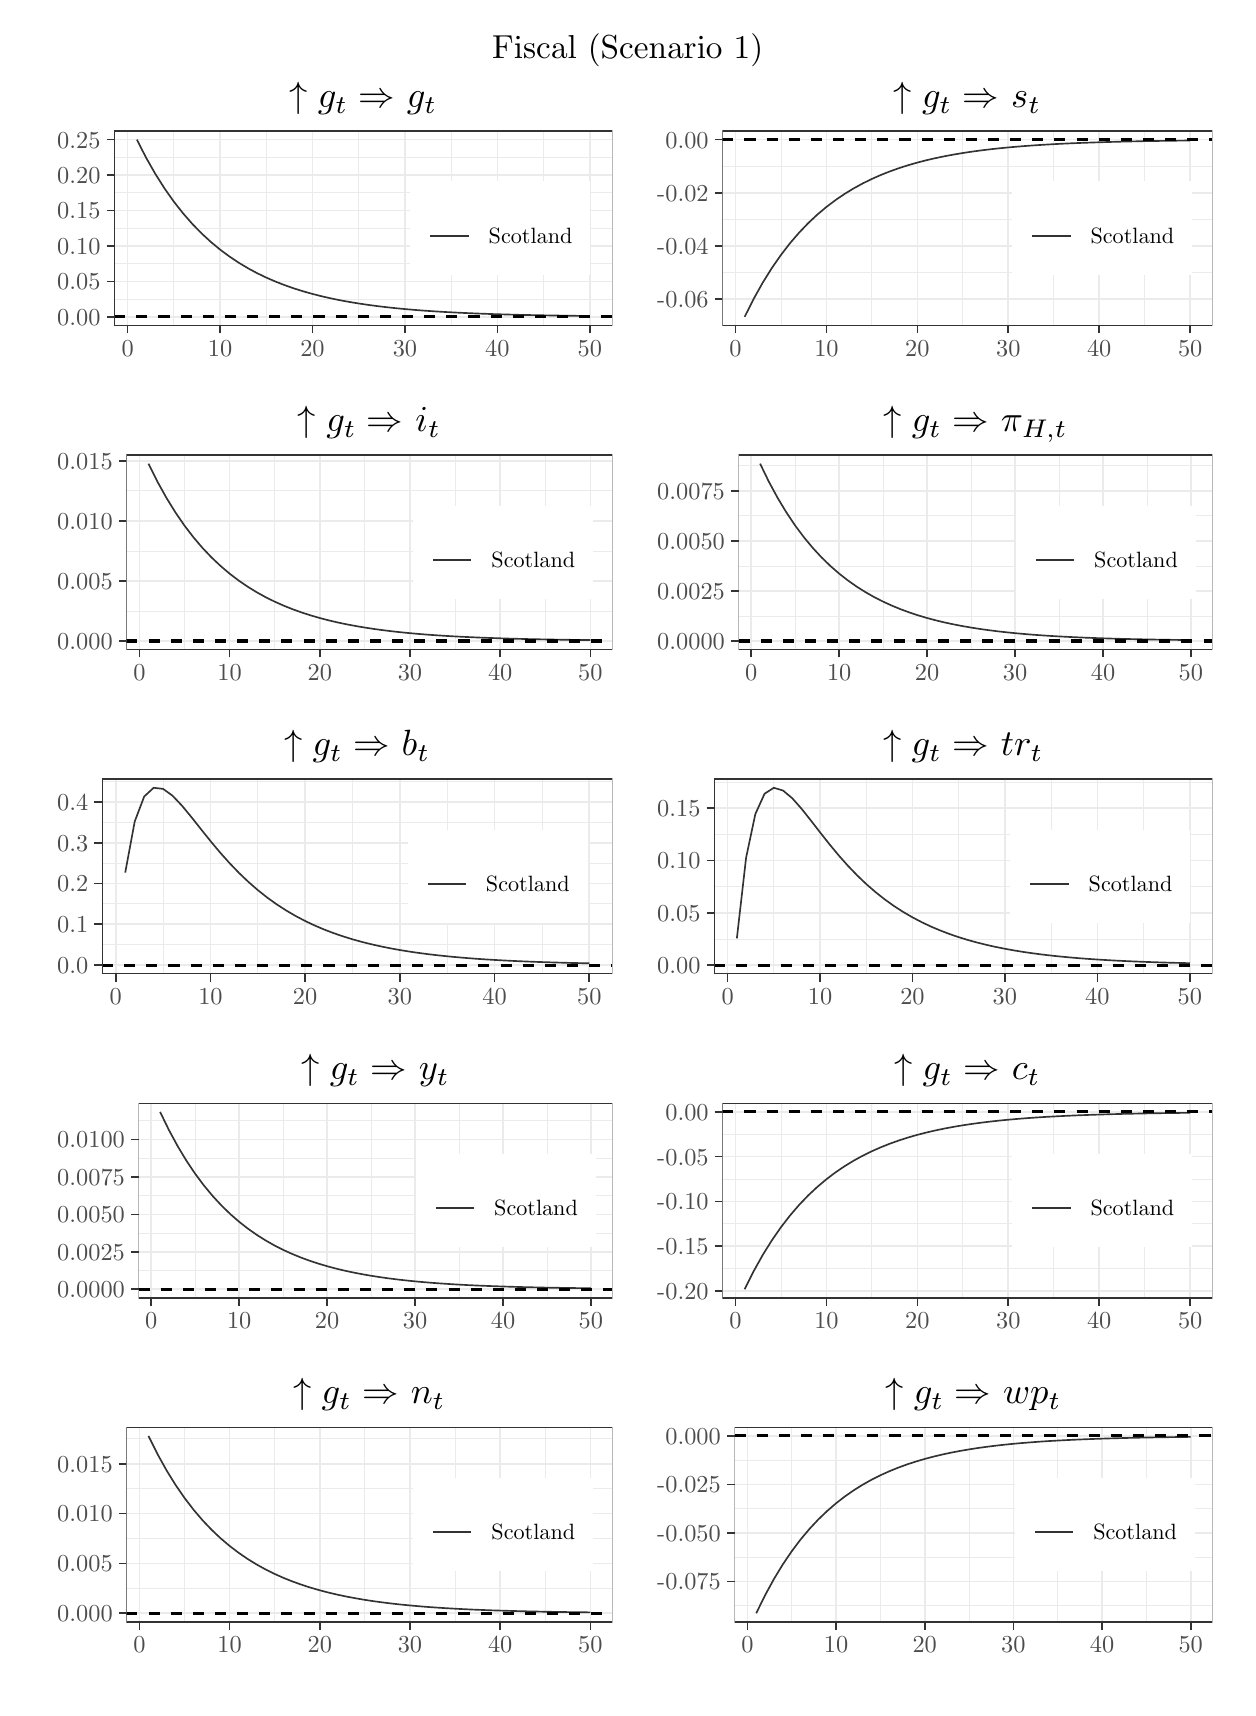
\begin{tikzpicture}[x=1pt,y=1pt]
\definecolor{fillColor}{RGB}{255,255,255}
\path[use as bounding box,fill=fillColor,fill opacity=0.00] (0,0) rectangle (433.62,599.84);
\begin{scope}
\path[clip] (  0.00,468.44) rectangle (216.81,585.55);
\definecolor{drawColor}{RGB}{255,255,255}
\definecolor{fillColor}{RGB}{255,255,255}

\path[draw=drawColor,line width= 0.6pt,line join=round,line cap=round,fill=fillColor] (  0.00,468.44) rectangle (216.81,585.55);
\end{scope}
\begin{scope}
\path[clip] ( 31.27,492.12) rectangle (211.31,562.59);
\definecolor{fillColor}{RGB}{255,255,255}

\path[fill=fillColor] ( 31.27,492.12) rectangle (211.31,562.59);
\definecolor{drawColor}{gray}{0.92}

\path[draw=drawColor,line width= 0.3pt,line join=round] ( 31.27,501.73) --
	(211.31,501.73);

\path[draw=drawColor,line width= 0.3pt,line join=round] ( 31.27,514.54) --
	(211.31,514.54);

\path[draw=drawColor,line width= 0.3pt,line join=round] ( 31.27,527.36) --
	(211.31,527.36);

\path[draw=drawColor,line width= 0.3pt,line join=round] ( 31.27,540.17) --
	(211.31,540.17);

\path[draw=drawColor,line width= 0.3pt,line join=round] ( 31.27,552.98) --
	(211.31,552.98);

\path[draw=drawColor,line width= 0.3pt,line join=round] ( 52.81,492.12) --
	( 52.81,562.59);

\path[draw=drawColor,line width= 0.3pt,line join=round] ( 86.22,492.12) --
	( 86.22,562.59);

\path[draw=drawColor,line width= 0.3pt,line join=round] (119.62,492.12) --
	(119.62,562.59);

\path[draw=drawColor,line width= 0.3pt,line join=round] (153.02,492.12) --
	(153.02,562.59);

\path[draw=drawColor,line width= 0.3pt,line join=round] (186.43,492.12) --
	(186.43,562.59);

\path[draw=drawColor,line width= 0.6pt,line join=round] ( 31.27,495.32) --
	(211.31,495.32);

\path[draw=drawColor,line width= 0.6pt,line join=round] ( 31.27,508.14) --
	(211.31,508.14);

\path[draw=drawColor,line width= 0.6pt,line join=round] ( 31.27,520.95) --
	(211.31,520.95);

\path[draw=drawColor,line width= 0.6pt,line join=round] ( 31.27,533.76) --
	(211.31,533.76);

\path[draw=drawColor,line width= 0.6pt,line join=round] ( 31.27,546.58) --
	(211.31,546.58);

\path[draw=drawColor,line width= 0.6pt,line join=round] ( 31.27,559.39) --
	(211.31,559.39);

\path[draw=drawColor,line width= 0.6pt,line join=round] ( 36.11,492.12) --
	( 36.11,562.59);

\path[draw=drawColor,line width= 0.6pt,line join=round] ( 69.52,492.12) --
	( 69.52,562.59);

\path[draw=drawColor,line width= 0.6pt,line join=round] (102.92,492.12) --
	(102.92,562.59);

\path[draw=drawColor,line width= 0.6pt,line join=round] (136.32,492.12) --
	(136.32,562.59);

\path[draw=drawColor,line width= 0.6pt,line join=round] (169.72,492.12) --
	(169.72,562.59);

\path[draw=drawColor,line width= 0.6pt,line join=round] (203.13,492.12) --
	(203.13,562.59);
\definecolor{drawColor}{gray}{0.20}

\path[draw=drawColor,line width= 0.6pt,line join=round] ( 39.45,559.39) --
	( 42.79,552.85) --
	( 46.13,546.99) --
	( 49.47,541.72) --
	( 52.81,536.98) --
	( 56.15,532.74) --
	( 59.50,528.92) --
	( 62.84,525.49) --
	( 66.18,522.42) --
	( 69.52,519.65) --
	( 72.86,517.17) --
	( 76.20,514.94) --
	( 79.54,512.94) --
	( 82.88,511.14) --
	( 86.22,509.53) --
	( 89.56,508.08) --
	( 92.90,506.78) --
	( 96.24,505.61) --
	( 99.58,504.56) --
	(102.92,503.62) --
	(106.26,502.77) --
	(109.60,502.01) --
	(112.94,501.33) --
	(116.28,500.72) --
	(119.62,500.17) --
	(122.96,499.67) --
	(126.30,499.23) --
	(129.64,498.83) --
	(132.98,498.47) --
	(136.32,498.15) --
	(139.66,497.86) --
	(143.00,497.60) --
	(146.34,497.37) --
	(149.68,497.16) --
	(153.02,496.98) --
	(156.36,496.81) --
	(159.70,496.66) --
	(163.04,496.52) --
	(166.38,496.40) --
	(169.72,496.29) --
	(173.06,496.19) --
	(176.40,496.10) --
	(179.74,496.02) --
	(183.08,495.95) --
	(186.43,495.89) --
	(189.77,495.83) --
	(193.11,495.78) --
	(196.45,495.73) --
	(199.79,495.69) --
	(203.13,495.65);
\definecolor{drawColor}{RGB}{0,0,0}

\path[draw=drawColor,line width= 1.1pt,dash pattern=on 4pt off 4pt ,line join=round] ( 31.27,495.32) -- (211.31,495.32);
\definecolor{drawColor}{gray}{0.20}

\path[draw=drawColor,line width= 0.6pt,line join=round,line cap=round] ( 31.27,492.12) rectangle (211.31,562.59);
\end{scope}
\begin{scope}
\path[clip] (  0.00,  0.00) rectangle (433.62,599.84);
\definecolor{drawColor}{gray}{0.30}

\node[text=drawColor,anchor=base east,inner sep=0pt, outer sep=0pt, scale=  0.88] at ( 26.32,492.29) {0.00};

\node[text=drawColor,anchor=base east,inner sep=0pt, outer sep=0pt, scale=  0.88] at ( 26.32,505.11) {0.05};

\node[text=drawColor,anchor=base east,inner sep=0pt, outer sep=0pt, scale=  0.88] at ( 26.32,517.92) {0.10};

\node[text=drawColor,anchor=base east,inner sep=0pt, outer sep=0pt, scale=  0.88] at ( 26.32,530.73) {0.15};

\node[text=drawColor,anchor=base east,inner sep=0pt, outer sep=0pt, scale=  0.88] at ( 26.32,543.55) {0.20};

\node[text=drawColor,anchor=base east,inner sep=0pt, outer sep=0pt, scale=  0.88] at ( 26.32,556.36) {0.25};
\end{scope}
\begin{scope}
\path[clip] (  0.00,  0.00) rectangle (433.62,599.84);
\definecolor{drawColor}{gray}{0.20}

\path[draw=drawColor,line width= 0.6pt,line join=round] ( 28.52,495.32) --
	( 31.27,495.32);

\path[draw=drawColor,line width= 0.6pt,line join=round] ( 28.52,508.14) --
	( 31.27,508.14);

\path[draw=drawColor,line width= 0.6pt,line join=round] ( 28.52,520.95) --
	( 31.27,520.95);

\path[draw=drawColor,line width= 0.6pt,line join=round] ( 28.52,533.76) --
	( 31.27,533.76);

\path[draw=drawColor,line width= 0.6pt,line join=round] ( 28.52,546.58) --
	( 31.27,546.58);

\path[draw=drawColor,line width= 0.6pt,line join=round] ( 28.52,559.39) --
	( 31.27,559.39);
\end{scope}
\begin{scope}
\path[clip] (  0.00,  0.00) rectangle (433.62,599.84);
\definecolor{drawColor}{gray}{0.20}

\path[draw=drawColor,line width= 0.6pt,line join=round] ( 36.11,489.37) --
	( 36.11,492.12);

\path[draw=drawColor,line width= 0.6pt,line join=round] ( 69.52,489.37) --
	( 69.52,492.12);

\path[draw=drawColor,line width= 0.6pt,line join=round] (102.92,489.37) --
	(102.92,492.12);

\path[draw=drawColor,line width= 0.6pt,line join=round] (136.32,489.37) --
	(136.32,492.12);

\path[draw=drawColor,line width= 0.6pt,line join=round] (169.72,489.37) --
	(169.72,492.12);

\path[draw=drawColor,line width= 0.6pt,line join=round] (203.13,489.37) --
	(203.13,492.12);
\end{scope}
\begin{scope}
\path[clip] (  0.00,  0.00) rectangle (433.62,599.84);
\definecolor{drawColor}{gray}{0.30}

\node[text=drawColor,anchor=base,inner sep=0pt, outer sep=0pt, scale=  0.88] at ( 36.11,481.11) {0};

\node[text=drawColor,anchor=base,inner sep=0pt, outer sep=0pt, scale=  0.88] at ( 69.52,481.11) {10};

\node[text=drawColor,anchor=base,inner sep=0pt, outer sep=0pt, scale=  0.88] at (102.92,481.11) {20};

\node[text=drawColor,anchor=base,inner sep=0pt, outer sep=0pt, scale=  0.88] at (136.32,481.11) {30};

\node[text=drawColor,anchor=base,inner sep=0pt, outer sep=0pt, scale=  0.88] at (169.72,481.11) {40};

\node[text=drawColor,anchor=base,inner sep=0pt, outer sep=0pt, scale=  0.88] at (203.13,481.11) {50};
\end{scope}
\begin{scope}
\path[clip] (  0.00,  0.00) rectangle (433.62,599.84);
\definecolor{fillColor}{RGB}{255,255,255}

\path[fill=fillColor] (138.26,510.43) rectangle (203.35,544.28);
\end{scope}
\begin{scope}
\path[clip] (  0.00,  0.00) rectangle (433.62,599.84);
\definecolor{fillColor}{RGB}{255,255,255}

\path[fill=fillColor] (143.76,515.93) rectangle (161.10,533.28);
\end{scope}
\begin{scope}
\path[clip] (  0.00,  0.00) rectangle (433.62,599.84);
\definecolor{drawColor}{gray}{0.20}

\path[draw=drawColor,line width= 0.6pt,line join=round] (145.49,524.61) -- (159.37,524.61);
\end{scope}
\begin{scope}
\path[clip] (  0.00,  0.00) rectangle (433.62,599.84);
\definecolor{drawColor}{RGB}{0,0,0}

\node[text=drawColor,anchor=base west,inner sep=0pt, outer sep=0pt, scale=  0.80] at (166.60,521.85) {Scotland};
\end{scope}
\begin{scope}
\path[clip] (  0.00,  0.00) rectangle (433.62,599.84);
\definecolor{drawColor}{RGB}{0,0,0}

\node[text=drawColor,anchor=base,inner sep=0pt, outer sep=0pt, scale=  1.32] at (121.29,570.96) {$\uparrow  g_t \Rightarrow $ ${g_t}$};
\end{scope}
\begin{scope}
\path[clip] (216.81,468.44) rectangle (433.62,585.55);
\definecolor{drawColor}{RGB}{255,255,255}
\definecolor{fillColor}{RGB}{255,255,255}

\path[draw=drawColor,line width= 0.6pt,line join=round,line cap=round,fill=fillColor] (216.81,468.44) rectangle (433.62,585.55);
\end{scope}
\begin{scope}
\path[clip] (251.01,492.12) rectangle (428.12,562.59);
\definecolor{fillColor}{RGB}{255,255,255}

\path[fill=fillColor] (251.01,492.12) rectangle (428.12,562.59);
\definecolor{drawColor}{gray}{0.92}

\path[draw=drawColor,line width= 0.3pt,line join=round] (251.01,492.25) --
	(428.12,492.25);

\path[draw=drawColor,line width= 0.3pt,line join=round] (251.01,511.43) --
	(428.12,511.43);

\path[draw=drawColor,line width= 0.3pt,line join=round] (251.01,530.61) --
	(428.12,530.61);

\path[draw=drawColor,line width= 0.3pt,line join=round] (251.01,549.80) --
	(428.12,549.80);

\path[draw=drawColor,line width= 0.3pt,line join=round] (272.21,492.12) --
	(272.21,562.59);

\path[draw=drawColor,line width= 0.3pt,line join=round] (305.06,492.12) --
	(305.06,562.59);

\path[draw=drawColor,line width= 0.3pt,line join=round] (337.92,492.12) --
	(337.92,562.59);

\path[draw=drawColor,line width= 0.3pt,line join=round] (370.78,492.12) --
	(370.78,562.59);

\path[draw=drawColor,line width= 0.3pt,line join=round] (403.64,492.12) --
	(403.64,562.59);

\path[draw=drawColor,line width= 0.6pt,line join=round] (251.01,501.84) --
	(428.12,501.84);

\path[draw=drawColor,line width= 0.6pt,line join=round] (251.01,521.02) --
	(428.12,521.02);

\path[draw=drawColor,line width= 0.6pt,line join=round] (251.01,540.21) --
	(428.12,540.21);

\path[draw=drawColor,line width= 0.6pt,line join=round] (251.01,559.39) --
	(428.12,559.39);

\path[draw=drawColor,line width= 0.6pt,line join=round] (255.78,492.12) --
	(255.78,562.59);

\path[draw=drawColor,line width= 0.6pt,line join=round] (288.64,492.12) --
	(288.64,562.59);

\path[draw=drawColor,line width= 0.6pt,line join=round] (321.49,492.12) --
	(321.49,562.59);

\path[draw=drawColor,line width= 0.6pt,line join=round] (354.35,492.12) --
	(354.35,562.59);

\path[draw=drawColor,line width= 0.6pt,line join=round] (387.21,492.12) --
	(387.21,562.59);

\path[draw=drawColor,line width= 0.6pt,line join=round] (420.07,492.12) --
	(420.07,562.59);
\definecolor{drawColor}{gray}{0.20}

\path[draw=drawColor,line width= 0.6pt,line join=round] (259.06,495.32) --
	(262.35,501.86) --
	(265.63,507.73) --
	(268.92,513.00) --
	(272.21,517.73) --
	(275.49,521.98) --
	(278.78,525.79) --
	(282.06,529.22) --
	(285.35,532.30) --
	(288.64,535.06) --
	(291.92,537.54) --
	(295.21,539.77) --
	(298.49,541.77) --
	(301.78,543.57) --
	(305.06,545.18) --
	(308.35,546.63) --
	(311.64,547.93) --
	(314.92,549.10) --
	(318.21,550.15) --
	(321.49,551.09) --
	(324.78,551.94) --
	(328.07,552.70) --
	(331.35,553.38) --
	(334.64,553.99) --
	(337.92,554.54) --
	(341.21,555.04) --
	(344.49,555.48) --
	(347.78,555.88) --
	(351.07,556.24) --
	(354.35,556.56) --
	(357.64,556.85) --
	(360.92,557.11) --
	(364.21,557.34) --
	(367.50,557.55) --
	(370.78,557.74) --
	(374.07,557.91) --
	(377.35,558.06) --
	(380.64,558.19) --
	(383.93,558.31) --
	(387.21,558.42) --
	(390.50,558.52) --
	(393.78,558.61) --
	(397.07,558.69) --
	(400.35,558.76) --
	(403.64,558.83) --
	(406.93,558.88) --
	(410.21,558.93) --
	(413.50,558.98) --
	(416.78,559.02) --
	(420.07,559.06);
\definecolor{drawColor}{RGB}{0,0,0}

\path[draw=drawColor,line width= 1.1pt,dash pattern=on 4pt off 4pt ,line join=round] (251.01,559.39) -- (428.12,559.39);
\definecolor{drawColor}{gray}{0.20}

\path[draw=drawColor,line width= 0.6pt,line join=round,line cap=round] (251.01,492.12) rectangle (428.12,562.59);
\end{scope}
\begin{scope}
\path[clip] (  0.00,  0.00) rectangle (433.62,599.84);
\definecolor{drawColor}{gray}{0.30}

\node[text=drawColor,anchor=base east,inner sep=0pt, outer sep=0pt, scale=  0.88] at (246.06,498.81) {-0.06};

\node[text=drawColor,anchor=base east,inner sep=0pt, outer sep=0pt, scale=  0.88] at (246.06,517.99) {-0.04};

\node[text=drawColor,anchor=base east,inner sep=0pt, outer sep=0pt, scale=  0.88] at (246.06,537.17) {-0.02};

\node[text=drawColor,anchor=base east,inner sep=0pt, outer sep=0pt, scale=  0.88] at (246.06,556.36) {0.00};
\end{scope}
\begin{scope}
\path[clip] (  0.00,  0.00) rectangle (433.62,599.84);
\definecolor{drawColor}{gray}{0.20}

\path[draw=drawColor,line width= 0.6pt,line join=round] (248.26,501.84) --
	(251.01,501.84);

\path[draw=drawColor,line width= 0.6pt,line join=round] (248.26,521.02) --
	(251.01,521.02);

\path[draw=drawColor,line width= 0.6pt,line join=round] (248.26,540.21) --
	(251.01,540.21);

\path[draw=drawColor,line width= 0.6pt,line join=round] (248.26,559.39) --
	(251.01,559.39);
\end{scope}
\begin{scope}
\path[clip] (  0.00,  0.00) rectangle (433.62,599.84);
\definecolor{drawColor}{gray}{0.20}

\path[draw=drawColor,line width= 0.6pt,line join=round] (255.78,489.37) --
	(255.78,492.12);

\path[draw=drawColor,line width= 0.6pt,line join=round] (288.64,489.37) --
	(288.64,492.12);

\path[draw=drawColor,line width= 0.6pt,line join=round] (321.49,489.37) --
	(321.49,492.12);

\path[draw=drawColor,line width= 0.6pt,line join=round] (354.35,489.37) --
	(354.35,492.12);

\path[draw=drawColor,line width= 0.6pt,line join=round] (387.21,489.37) --
	(387.21,492.12);

\path[draw=drawColor,line width= 0.6pt,line join=round] (420.07,489.37) --
	(420.07,492.12);
\end{scope}
\begin{scope}
\path[clip] (  0.00,  0.00) rectangle (433.62,599.84);
\definecolor{drawColor}{gray}{0.30}

\node[text=drawColor,anchor=base,inner sep=0pt, outer sep=0pt, scale=  0.88] at (255.78,481.11) {0};

\node[text=drawColor,anchor=base,inner sep=0pt, outer sep=0pt, scale=  0.88] at (288.64,481.11) {10};

\node[text=drawColor,anchor=base,inner sep=0pt, outer sep=0pt, scale=  0.88] at (321.49,481.11) {20};

\node[text=drawColor,anchor=base,inner sep=0pt, outer sep=0pt, scale=  0.88] at (354.35,481.11) {30};

\node[text=drawColor,anchor=base,inner sep=0pt, outer sep=0pt, scale=  0.88] at (387.21,481.11) {40};

\node[text=drawColor,anchor=base,inner sep=0pt, outer sep=0pt, scale=  0.88] at (420.07,481.11) {50};
\end{scope}
\begin{scope}
\path[clip] (  0.00,  0.00) rectangle (433.62,599.84);
\definecolor{fillColor}{RGB}{255,255,255}

\path[fill=fillColor] (355.73,510.43) rectangle (420.82,544.28);
\end{scope}
\begin{scope}
\path[clip] (  0.00,  0.00) rectangle (433.62,599.84);
\definecolor{fillColor}{RGB}{255,255,255}

\path[fill=fillColor] (361.23,515.93) rectangle (378.57,533.28);
\end{scope}
\begin{scope}
\path[clip] (  0.00,  0.00) rectangle (433.62,599.84);
\definecolor{drawColor}{gray}{0.20}

\path[draw=drawColor,line width= 0.6pt,line join=round] (362.96,524.61) -- (376.84,524.61);
\end{scope}
\begin{scope}
\path[clip] (  0.00,  0.00) rectangle (433.62,599.84);
\definecolor{drawColor}{RGB}{0,0,0}

\node[text=drawColor,anchor=base west,inner sep=0pt, outer sep=0pt, scale=  0.80] at (384.07,521.85) {Scotland};
\end{scope}
\begin{scope}
\path[clip] (  0.00,  0.00) rectangle (433.62,599.84);
\definecolor{drawColor}{RGB}{0,0,0}

\node[text=drawColor,anchor=base,inner sep=0pt, outer sep=0pt, scale=  1.32] at (339.57,570.96) {$\uparrow  g_t \Rightarrow $ ${s_t}$};
\end{scope}
\begin{scope}
\path[clip] (  0.00,351.33) rectangle (216.81,468.44);
\definecolor{drawColor}{RGB}{255,255,255}
\definecolor{fillColor}{RGB}{255,255,255}

\path[draw=drawColor,line width= 0.6pt,line join=round,line cap=round,fill=fillColor] (  0.00,351.33) rectangle (216.81,468.44);
\end{scope}
\begin{scope}
\path[clip] ( 35.67,375.01) rectangle (211.31,445.48);
\definecolor{fillColor}{RGB}{255,255,255}

\path[fill=fillColor] ( 35.67,375.01) rectangle (211.31,445.48);
\definecolor{drawColor}{gray}{0.92}

\path[draw=drawColor,line width= 0.3pt,line join=round] ( 35.67,389.06) --
	(211.31,389.06);

\path[draw=drawColor,line width= 0.3pt,line join=round] ( 35.67,410.76) --
	(211.31,410.76);

\path[draw=drawColor,line width= 0.3pt,line join=round] ( 35.67,432.45) --
	(211.31,432.45);

\path[draw=drawColor,line width= 0.3pt,line join=round] ( 56.69,375.01) --
	( 56.69,445.48);

\path[draw=drawColor,line width= 0.3pt,line join=round] ( 89.27,375.01) --
	( 89.27,445.48);

\path[draw=drawColor,line width= 0.3pt,line join=round] (121.86,375.01) --
	(121.86,445.48);

\path[draw=drawColor,line width= 0.3pt,line join=round] (154.45,375.01) --
	(154.45,445.48);

\path[draw=drawColor,line width= 0.3pt,line join=round] (187.03,375.01) --
	(187.03,445.48);

\path[draw=drawColor,line width= 0.6pt,line join=round] ( 35.67,378.21) --
	(211.31,378.21);

\path[draw=drawColor,line width= 0.6pt,line join=round] ( 35.67,399.91) --
	(211.31,399.91);

\path[draw=drawColor,line width= 0.6pt,line join=round] ( 35.67,421.60) --
	(211.31,421.60);

\path[draw=drawColor,line width= 0.6pt,line join=round] ( 35.67,443.30) --
	(211.31,443.30);

\path[draw=drawColor,line width= 0.6pt,line join=round] ( 40.39,375.01) --
	( 40.39,445.48);

\path[draw=drawColor,line width= 0.6pt,line join=round] ( 72.98,375.01) --
	( 72.98,445.48);

\path[draw=drawColor,line width= 0.6pt,line join=round] (105.57,375.01) --
	(105.57,445.48);

\path[draw=drawColor,line width= 0.6pt,line join=round] (138.15,375.01) --
	(138.15,445.48);

\path[draw=drawColor,line width= 0.6pt,line join=round] (170.74,375.01) --
	(170.74,445.48);

\path[draw=drawColor,line width= 0.6pt,line join=round] (203.33,375.01) --
	(203.33,445.48);
\definecolor{drawColor}{gray}{0.20}

\path[draw=drawColor,line width= 0.6pt,line join=round] ( 43.65,442.28) --
	( 46.91,435.74) --
	( 50.17,429.88) --
	( 53.43,424.61) --
	( 56.69,419.87) --
	( 59.95,415.62) --
	( 63.20,411.81) --
	( 66.46,408.38) --
	( 69.72,405.31) --
	( 72.98,402.54) --
	( 76.24,400.06) --
	( 79.50,397.83) --
	( 82.76,395.83) --
	( 86.01,394.03) --
	( 89.27,392.42) --
	( 92.53,390.97) --
	( 95.79,389.67) --
	( 99.05,388.50) --
	(102.31,387.45) --
	(105.57,386.51) --
	(108.83,385.66) --
	(112.08,384.90) --
	(115.34,384.22) --
	(118.60,383.61) --
	(121.86,383.06) --
	(125.12,382.56) --
	(128.38,382.12) --
	(131.64,381.72) --
	(134.89,381.36) --
	(138.15,381.04) --
	(141.41,380.75) --
	(144.67,380.49) --
	(147.93,380.26) --
	(151.19,380.05) --
	(154.45,379.86) --
	(157.71,379.70) --
	(160.96,379.55) --
	(164.22,379.41) --
	(167.48,379.29) --
	(170.74,379.18) --
	(174.00,379.08) --
	(177.26,378.99) --
	(180.52,378.91) --
	(183.77,378.84) --
	(187.03,378.78) --
	(190.29,378.72) --
	(193.55,378.67) --
	(196.81,378.62) --
	(200.07,378.58) --
	(203.33,378.54);
\definecolor{drawColor}{RGB}{0,0,0}

\path[draw=drawColor,line width= 1.1pt,dash pattern=on 4pt off 4pt ,line join=round] ( 35.67,378.21) -- (211.31,378.21);
\definecolor{drawColor}{gray}{0.20}

\path[draw=drawColor,line width= 0.6pt,line join=round,line cap=round] ( 35.67,375.01) rectangle (211.31,445.48);
\end{scope}
\begin{scope}
\path[clip] (  0.00,  0.00) rectangle (433.62,599.84);
\definecolor{drawColor}{gray}{0.30}

\node[text=drawColor,anchor=base east,inner sep=0pt, outer sep=0pt, scale=  0.88] at ( 30.72,375.18) {0.000};

\node[text=drawColor,anchor=base east,inner sep=0pt, outer sep=0pt, scale=  0.88] at ( 30.72,396.88) {0.005};

\node[text=drawColor,anchor=base east,inner sep=0pt, outer sep=0pt, scale=  0.88] at ( 30.72,418.57) {0.010};

\node[text=drawColor,anchor=base east,inner sep=0pt, outer sep=0pt, scale=  0.88] at ( 30.72,440.27) {0.015};
\end{scope}
\begin{scope}
\path[clip] (  0.00,  0.00) rectangle (433.62,599.84);
\definecolor{drawColor}{gray}{0.20}

\path[draw=drawColor,line width= 0.6pt,line join=round] ( 32.92,378.21) --
	( 35.67,378.21);

\path[draw=drawColor,line width= 0.6pt,line join=round] ( 32.92,399.91) --
	( 35.67,399.91);

\path[draw=drawColor,line width= 0.6pt,line join=round] ( 32.92,421.60) --
	( 35.67,421.60);

\path[draw=drawColor,line width= 0.6pt,line join=round] ( 32.92,443.30) --
	( 35.67,443.30);
\end{scope}
\begin{scope}
\path[clip] (  0.00,  0.00) rectangle (433.62,599.84);
\definecolor{drawColor}{gray}{0.20}

\path[draw=drawColor,line width= 0.6pt,line join=round] ( 40.39,372.26) --
	( 40.39,375.01);

\path[draw=drawColor,line width= 0.6pt,line join=round] ( 72.98,372.26) --
	( 72.98,375.01);

\path[draw=drawColor,line width= 0.6pt,line join=round] (105.57,372.26) --
	(105.57,375.01);

\path[draw=drawColor,line width= 0.6pt,line join=round] (138.15,372.26) --
	(138.15,375.01);

\path[draw=drawColor,line width= 0.6pt,line join=round] (170.74,372.26) --
	(170.74,375.01);

\path[draw=drawColor,line width= 0.6pt,line join=round] (203.33,372.26) --
	(203.33,375.01);
\end{scope}
\begin{scope}
\path[clip] (  0.00,  0.00) rectangle (433.62,599.84);
\definecolor{drawColor}{gray}{0.30}

\node[text=drawColor,anchor=base,inner sep=0pt, outer sep=0pt, scale=  0.88] at ( 40.39,364.00) {0};

\node[text=drawColor,anchor=base,inner sep=0pt, outer sep=0pt, scale=  0.88] at ( 72.98,364.00) {10};

\node[text=drawColor,anchor=base,inner sep=0pt, outer sep=0pt, scale=  0.88] at (105.57,364.00) {20};

\node[text=drawColor,anchor=base,inner sep=0pt, outer sep=0pt, scale=  0.88] at (138.15,364.00) {30};

\node[text=drawColor,anchor=base,inner sep=0pt, outer sep=0pt, scale=  0.88] at (170.74,364.00) {40};

\node[text=drawColor,anchor=base,inner sep=0pt, outer sep=0pt, scale=  0.88] at (203.33,364.00) {50};
\end{scope}
\begin{scope}
\path[clip] (  0.00,  0.00) rectangle (433.62,599.84);
\definecolor{fillColor}{RGB}{255,255,255}

\path[fill=fillColor] (139.25,393.32) rectangle (204.34,427.17);
\end{scope}
\begin{scope}
\path[clip] (  0.00,  0.00) rectangle (433.62,599.84);
\definecolor{fillColor}{RGB}{255,255,255}

\path[fill=fillColor] (144.75,398.82) rectangle (162.09,416.17);
\end{scope}
\begin{scope}
\path[clip] (  0.00,  0.00) rectangle (433.62,599.84);
\definecolor{drawColor}{gray}{0.20}

\path[draw=drawColor,line width= 0.6pt,line join=round] (146.48,407.50) -- (160.36,407.50);
\end{scope}
\begin{scope}
\path[clip] (  0.00,  0.00) rectangle (433.62,599.84);
\definecolor{drawColor}{RGB}{0,0,0}

\node[text=drawColor,anchor=base west,inner sep=0pt, outer sep=0pt, scale=  0.80] at (167.59,404.74) {Scotland};
\end{scope}
\begin{scope}
\path[clip] (  0.00,  0.00) rectangle (433.62,599.84);
\definecolor{drawColor}{RGB}{0,0,0}

\node[text=drawColor,anchor=base,inner sep=0pt, outer sep=0pt, scale=  1.32] at (123.49,453.85) {$\uparrow  g_t \Rightarrow $ ${i_t}$};
\end{scope}
\begin{scope}
\path[clip] (216.81,351.33) rectangle (433.62,468.44);
\definecolor{drawColor}{RGB}{255,255,255}
\definecolor{fillColor}{RGB}{255,255,255}

\path[draw=drawColor,line width= 0.6pt,line join=round,line cap=round,fill=fillColor] (216.81,351.33) rectangle (433.62,468.44);
\end{scope}
\begin{scope}
\path[clip] (256.88,375.01) rectangle (428.12,445.48);
\definecolor{fillColor}{RGB}{255,255,255}

\path[fill=fillColor] (256.88,375.01) rectangle (428.12,445.48);
\definecolor{drawColor}{gray}{0.92}

\path[draw=drawColor,line width= 0.3pt,line join=round] (256.88,387.26) --
	(428.12,387.26);

\path[draw=drawColor,line width= 0.3pt,line join=round] (256.88,405.34) --
	(428.12,405.34);

\path[draw=drawColor,line width= 0.3pt,line join=round] (256.88,423.43) --
	(428.12,423.43);

\path[draw=drawColor,line width= 0.3pt,line join=round] (256.88,441.51) --
	(428.12,441.51);

\path[draw=drawColor,line width= 0.3pt,line join=round] (277.37,375.01) --
	(277.37,445.48);

\path[draw=drawColor,line width= 0.3pt,line join=round] (309.14,375.01) --
	(309.14,445.48);

\path[draw=drawColor,line width= 0.3pt,line join=round] (340.91,375.01) --
	(340.91,445.48);

\path[draw=drawColor,line width= 0.3pt,line join=round] (372.68,375.01) --
	(372.68,445.48);

\path[draw=drawColor,line width= 0.3pt,line join=round] (404.45,375.01) --
	(404.45,445.48);

\path[draw=drawColor,line width= 0.6pt,line join=round] (256.88,378.21) --
	(428.12,378.21);

\path[draw=drawColor,line width= 0.6pt,line join=round] (256.88,396.30) --
	(428.12,396.30);

\path[draw=drawColor,line width= 0.6pt,line join=round] (256.88,414.38) --
	(428.12,414.38);

\path[draw=drawColor,line width= 0.6pt,line join=round] (256.88,432.47) --
	(428.12,432.47);

\path[draw=drawColor,line width= 0.6pt,line join=round] (261.48,375.01) --
	(261.48,445.48);

\path[draw=drawColor,line width= 0.6pt,line join=round] (293.25,375.01) --
	(293.25,445.48);

\path[draw=drawColor,line width= 0.6pt,line join=round] (325.03,375.01) --
	(325.03,445.48);

\path[draw=drawColor,line width= 0.6pt,line join=round] (356.80,375.01) --
	(356.80,445.48);

\path[draw=drawColor,line width= 0.6pt,line join=round] (388.57,375.01) --
	(388.57,445.48);

\path[draw=drawColor,line width= 0.6pt,line join=round] (420.34,375.01) --
	(420.34,445.48);
\definecolor{drawColor}{gray}{0.20}

\path[draw=drawColor,line width= 0.6pt,line join=round] (264.66,442.28) --
	(267.84,435.74) --
	(271.02,429.87) --
	(274.19,424.61) --
	(277.37,419.87) --
	(280.55,415.62) --
	(283.72,411.81) --
	(286.90,408.38) --
	(290.08,405.30) --
	(293.25,402.54) --
	(296.43,400.06) --
	(299.61,397.83) --
	(302.79,395.83) --
	(305.96,394.03) --
	(309.14,392.42) --
	(312.32,390.97) --
	(315.49,389.67) --
	(318.67,388.50) --
	(321.85,387.45) --
	(325.03,386.51) --
	(328.20,385.66) --
	(331.38,384.90) --
	(334.56,384.22) --
	(337.73,383.61) --
	(340.91,383.06) --
	(344.09,382.56) --
	(347.26,382.12) --
	(350.44,381.72) --
	(353.62,381.36) --
	(356.80,381.04) --
	(359.97,380.75) --
	(363.15,380.49) --
	(366.33,380.26) --
	(369.50,380.05) --
	(372.68,379.86) --
	(375.86,379.70) --
	(379.03,379.55) --
	(382.21,379.41) --
	(385.39,379.29) --
	(388.57,379.18) --
	(391.74,379.08) --
	(394.92,378.99) --
	(398.10,378.91) --
	(401.27,378.84) --
	(404.45,378.78) --
	(407.63,378.72) --
	(410.81,378.67) --
	(413.98,378.62) --
	(417.16,378.58) --
	(420.34,378.54);
\definecolor{drawColor}{RGB}{0,0,0}

\path[draw=drawColor,line width= 1.1pt,dash pattern=on 4pt off 4pt ,line join=round] (256.88,378.21) -- (428.12,378.21);
\definecolor{drawColor}{gray}{0.20}

\path[draw=drawColor,line width= 0.6pt,line join=round,line cap=round] (256.88,375.01) rectangle (428.12,445.48);
\end{scope}
\begin{scope}
\path[clip] (  0.00,  0.00) rectangle (433.62,599.84);
\definecolor{drawColor}{gray}{0.30}

\node[text=drawColor,anchor=base east,inner sep=0pt, outer sep=0pt, scale=  0.88] at (251.93,375.18) {0.0000};

\node[text=drawColor,anchor=base east,inner sep=0pt, outer sep=0pt, scale=  0.88] at (251.93,393.27) {0.0025};

\node[text=drawColor,anchor=base east,inner sep=0pt, outer sep=0pt, scale=  0.88] at (251.93,411.35) {0.0050};

\node[text=drawColor,anchor=base east,inner sep=0pt, outer sep=0pt, scale=  0.88] at (251.93,429.44) {0.0075};
\end{scope}
\begin{scope}
\path[clip] (  0.00,  0.00) rectangle (433.62,599.84);
\definecolor{drawColor}{gray}{0.20}

\path[draw=drawColor,line width= 0.6pt,line join=round] (254.13,378.21) --
	(256.88,378.21);

\path[draw=drawColor,line width= 0.6pt,line join=round] (254.13,396.30) --
	(256.88,396.30);

\path[draw=drawColor,line width= 0.6pt,line join=round] (254.13,414.38) --
	(256.88,414.38);

\path[draw=drawColor,line width= 0.6pt,line join=round] (254.13,432.47) --
	(256.88,432.47);
\end{scope}
\begin{scope}
\path[clip] (  0.00,  0.00) rectangle (433.62,599.84);
\definecolor{drawColor}{gray}{0.20}

\path[draw=drawColor,line width= 0.6pt,line join=round] (261.48,372.26) --
	(261.48,375.01);

\path[draw=drawColor,line width= 0.6pt,line join=round] (293.25,372.26) --
	(293.25,375.01);

\path[draw=drawColor,line width= 0.6pt,line join=round] (325.03,372.26) --
	(325.03,375.01);

\path[draw=drawColor,line width= 0.6pt,line join=round] (356.80,372.26) --
	(356.80,375.01);

\path[draw=drawColor,line width= 0.6pt,line join=round] (388.57,372.26) --
	(388.57,375.01);

\path[draw=drawColor,line width= 0.6pt,line join=round] (420.34,372.26) --
	(420.34,375.01);
\end{scope}
\begin{scope}
\path[clip] (  0.00,  0.00) rectangle (433.62,599.84);
\definecolor{drawColor}{gray}{0.30}

\node[text=drawColor,anchor=base,inner sep=0pt, outer sep=0pt, scale=  0.88] at (261.48,364.00) {0};

\node[text=drawColor,anchor=base,inner sep=0pt, outer sep=0pt, scale=  0.88] at (293.25,364.00) {10};

\node[text=drawColor,anchor=base,inner sep=0pt, outer sep=0pt, scale=  0.88] at (325.03,364.00) {20};

\node[text=drawColor,anchor=base,inner sep=0pt, outer sep=0pt, scale=  0.88] at (356.80,364.00) {30};

\node[text=drawColor,anchor=base,inner sep=0pt, outer sep=0pt, scale=  0.88] at (388.57,364.00) {40};

\node[text=drawColor,anchor=base,inner sep=0pt, outer sep=0pt, scale=  0.88] at (420.34,364.00) {50};
\end{scope}
\begin{scope}
\path[clip] (  0.00,  0.00) rectangle (433.62,599.84);
\definecolor{fillColor}{RGB}{255,255,255}

\path[fill=fillColor] (357.05,393.32) rectangle (422.14,427.17);
\end{scope}
\begin{scope}
\path[clip] (  0.00,  0.00) rectangle (433.62,599.84);
\definecolor{fillColor}{RGB}{255,255,255}

\path[fill=fillColor] (362.55,398.82) rectangle (379.89,416.17);
\end{scope}
\begin{scope}
\path[clip] (  0.00,  0.00) rectangle (433.62,599.84);
\definecolor{drawColor}{gray}{0.20}

\path[draw=drawColor,line width= 0.6pt,line join=round] (364.28,407.50) -- (378.16,407.50);
\end{scope}
\begin{scope}
\path[clip] (  0.00,  0.00) rectangle (433.62,599.84);
\definecolor{drawColor}{RGB}{0,0,0}

\node[text=drawColor,anchor=base west,inner sep=0pt, outer sep=0pt, scale=  0.80] at (385.39,404.74) {Scotland};
\end{scope}
\begin{scope}
\path[clip] (  0.00,  0.00) rectangle (433.62,599.84);
\definecolor{drawColor}{RGB}{0,0,0}

\node[text=drawColor,anchor=base,inner sep=0pt, outer sep=0pt, scale=  1.32] at (342.50,453.85) {$\uparrow  g_t \Rightarrow $ ${\pi_{H,t}}$};
\end{scope}
\begin{scope}
\path[clip] (  0.00,234.22) rectangle (216.81,351.33);
\definecolor{drawColor}{RGB}{255,255,255}
\definecolor{fillColor}{RGB}{255,255,255}

\path[draw=drawColor,line width= 0.6pt,line join=round,line cap=round,fill=fillColor] (  0.00,234.22) rectangle (216.81,351.33);
\end{scope}
\begin{scope}
\path[clip] ( 26.87,257.90) rectangle (211.31,328.37);
\definecolor{fillColor}{RGB}{255,255,255}

\path[fill=fillColor] ( 26.87,257.90) rectangle (211.31,328.37);
\definecolor{drawColor}{gray}{0.92}

\path[draw=drawColor,line width= 0.3pt,line join=round] ( 26.87,268.47) --
	(211.31,268.47);

\path[draw=drawColor,line width= 0.3pt,line join=round] ( 26.87,283.21) --
	(211.31,283.21);

\path[draw=drawColor,line width= 0.3pt,line join=round] ( 26.87,297.94) --
	(211.31,297.94);

\path[draw=drawColor,line width= 0.3pt,line join=round] ( 26.87,312.68) --
	(211.31,312.68);

\path[draw=drawColor,line width= 0.3pt,line join=round] ( 26.87,327.42) --
	(211.31,327.42);

\path[draw=drawColor,line width= 0.3pt,line join=round] ( 48.94,257.90) --
	( 48.94,328.37);

\path[draw=drawColor,line width= 0.3pt,line join=round] ( 83.16,257.90) --
	( 83.16,328.37);

\path[draw=drawColor,line width= 0.3pt,line join=round] (117.38,257.90) --
	(117.38,328.37);

\path[draw=drawColor,line width= 0.3pt,line join=round] (151.60,257.90) --
	(151.60,328.37);

\path[draw=drawColor,line width= 0.3pt,line join=round] (185.82,257.90) --
	(185.82,328.37);

\path[draw=drawColor,line width= 0.6pt,line join=round] ( 26.87,261.10) --
	(211.31,261.10);

\path[draw=drawColor,line width= 0.6pt,line join=round] ( 26.87,275.84) --
	(211.31,275.84);

\path[draw=drawColor,line width= 0.6pt,line join=round] ( 26.87,290.57) --
	(211.31,290.57);

\path[draw=drawColor,line width= 0.6pt,line join=round] ( 26.87,305.31) --
	(211.31,305.31);

\path[draw=drawColor,line width= 0.6pt,line join=round] ( 26.87,320.05) --
	(211.31,320.05);

\path[draw=drawColor,line width= 0.6pt,line join=round] ( 31.83,257.90) --
	( 31.83,328.37);

\path[draw=drawColor,line width= 0.6pt,line join=round] ( 66.05,257.90) --
	( 66.05,328.37);

\path[draw=drawColor,line width= 0.6pt,line join=round] (100.27,257.90) --
	(100.27,328.37);

\path[draw=drawColor,line width= 0.6pt,line join=round] (134.49,257.90) --
	(134.49,328.37);

\path[draw=drawColor,line width= 0.6pt,line join=round] (168.71,257.90) --
	(168.71,328.37);

\path[draw=drawColor,line width= 0.6pt,line join=round] (202.93,257.90) --
	(202.93,328.37);
\definecolor{drawColor}{gray}{0.20}

\path[draw=drawColor,line width= 0.6pt,line join=round] ( 35.25,294.52) --
	( 38.68,312.98) --
	( 42.10,322.01) --
	( 45.52,325.17) --
	( 48.94,324.77) --
	( 52.36,322.29) --
	( 55.79,318.67) --
	( 59.21,314.52) --
	( 62.63,310.20) --
	( 66.05,305.93) --
	( 69.47,301.84) --
	( 72.90,298.00) --
	( 76.32,294.44) --
	( 79.74,291.18) --
	( 83.16,288.20) --
	( 86.58,285.49) --
	( 90.00,283.04) --
	( 93.43,280.83) --
	( 96.85,278.83) --
	(100.27,277.04) --
	(103.69,275.42) --
	(107.11,273.96) --
	(110.54,272.65) --
	(113.96,271.48) --
	(117.38,270.42) --
	(120.80,269.47) --
	(124.22,268.62) --
	(127.65,267.85) --
	(131.07,267.16) --
	(134.49,266.54) --
	(137.91,265.99) --
	(141.33,265.49) --
	(144.75,265.04) --
	(148.18,264.64) --
	(151.60,264.28) --
	(155.02,263.96) --
	(158.44,263.67) --
	(161.86,263.40) --
	(165.29,263.17) --
	(168.71,262.96) --
	(172.13,262.77) --
	(175.55,262.60) --
	(178.97,262.45) --
	(182.40,262.31) --
	(185.82,262.19) --
	(189.24,262.08) --
	(192.66,261.98) --
	(196.08,261.89) --
	(199.50,261.81) --
	(202.93,261.74);
\definecolor{drawColor}{RGB}{0,0,0}

\path[draw=drawColor,line width= 1.1pt,dash pattern=on 4pt off 4pt ,line join=round] ( 26.87,261.10) -- (211.31,261.10);
\definecolor{drawColor}{gray}{0.20}

\path[draw=drawColor,line width= 0.6pt,line join=round,line cap=round] ( 26.87,257.90) rectangle (211.31,328.37);
\end{scope}
\begin{scope}
\path[clip] (  0.00,  0.00) rectangle (433.62,599.84);
\definecolor{drawColor}{gray}{0.30}

\node[text=drawColor,anchor=base east,inner sep=0pt, outer sep=0pt, scale=  0.88] at ( 21.92,258.07) {0.0};

\node[text=drawColor,anchor=base east,inner sep=0pt, outer sep=0pt, scale=  0.88] at ( 21.92,272.81) {0.1};

\node[text=drawColor,anchor=base east,inner sep=0pt, outer sep=0pt, scale=  0.88] at ( 21.92,287.54) {0.2};

\node[text=drawColor,anchor=base east,inner sep=0pt, outer sep=0pt, scale=  0.88] at ( 21.92,302.28) {0.3};

\node[text=drawColor,anchor=base east,inner sep=0pt, outer sep=0pt, scale=  0.88] at ( 21.92,317.02) {0.4};
\end{scope}
\begin{scope}
\path[clip] (  0.00,  0.00) rectangle (433.62,599.84);
\definecolor{drawColor}{gray}{0.20}

\path[draw=drawColor,line width= 0.6pt,line join=round] ( 24.12,261.10) --
	( 26.87,261.10);

\path[draw=drawColor,line width= 0.6pt,line join=round] ( 24.12,275.84) --
	( 26.87,275.84);

\path[draw=drawColor,line width= 0.6pt,line join=round] ( 24.12,290.57) --
	( 26.87,290.57);

\path[draw=drawColor,line width= 0.6pt,line join=round] ( 24.12,305.31) --
	( 26.87,305.31);

\path[draw=drawColor,line width= 0.6pt,line join=round] ( 24.12,320.05) --
	( 26.87,320.05);
\end{scope}
\begin{scope}
\path[clip] (  0.00,  0.00) rectangle (433.62,599.84);
\definecolor{drawColor}{gray}{0.20}

\path[draw=drawColor,line width= 0.6pt,line join=round] ( 31.83,255.15) --
	( 31.83,257.90);

\path[draw=drawColor,line width= 0.6pt,line join=round] ( 66.05,255.15) --
	( 66.05,257.90);

\path[draw=drawColor,line width= 0.6pt,line join=round] (100.27,255.15) --
	(100.27,257.90);

\path[draw=drawColor,line width= 0.6pt,line join=round] (134.49,255.15) --
	(134.49,257.90);

\path[draw=drawColor,line width= 0.6pt,line join=round] (168.71,255.15) --
	(168.71,257.90);

\path[draw=drawColor,line width= 0.6pt,line join=round] (202.93,255.15) --
	(202.93,257.90);
\end{scope}
\begin{scope}
\path[clip] (  0.00,  0.00) rectangle (433.62,599.84);
\definecolor{drawColor}{gray}{0.30}

\node[text=drawColor,anchor=base,inner sep=0pt, outer sep=0pt, scale=  0.88] at ( 31.83,246.89) {0};

\node[text=drawColor,anchor=base,inner sep=0pt, outer sep=0pt, scale=  0.88] at ( 66.05,246.89) {10};

\node[text=drawColor,anchor=base,inner sep=0pt, outer sep=0pt, scale=  0.88] at (100.27,246.89) {20};

\node[text=drawColor,anchor=base,inner sep=0pt, outer sep=0pt, scale=  0.88] at (134.49,246.89) {30};

\node[text=drawColor,anchor=base,inner sep=0pt, outer sep=0pt, scale=  0.88] at (168.71,246.89) {40};

\node[text=drawColor,anchor=base,inner sep=0pt, outer sep=0pt, scale=  0.88] at (202.93,246.89) {50};
\end{scope}
\begin{scope}
\path[clip] (  0.00,  0.00) rectangle (433.62,599.84);
\definecolor{fillColor}{RGB}{255,255,255}

\path[fill=fillColor] (137.27,276.21) rectangle (202.36,310.06);
\end{scope}
\begin{scope}
\path[clip] (  0.00,  0.00) rectangle (433.62,599.84);
\definecolor{fillColor}{RGB}{255,255,255}

\path[fill=fillColor] (142.77,281.71) rectangle (160.11,299.06);
\end{scope}
\begin{scope}
\path[clip] (  0.00,  0.00) rectangle (433.62,599.84);
\definecolor{drawColor}{gray}{0.20}

\path[draw=drawColor,line width= 0.6pt,line join=round] (144.50,290.38) -- (158.38,290.38);
\end{scope}
\begin{scope}
\path[clip] (  0.00,  0.00) rectangle (433.62,599.84);
\definecolor{drawColor}{RGB}{0,0,0}

\node[text=drawColor,anchor=base west,inner sep=0pt, outer sep=0pt, scale=  0.80] at (165.61,287.63) {Scotland};
\end{scope}
\begin{scope}
\path[clip] (  0.00,  0.00) rectangle (433.62,599.84);
\definecolor{drawColor}{RGB}{0,0,0}

\node[text=drawColor,anchor=base,inner sep=0pt, outer sep=0pt, scale=  1.32] at (119.09,336.74) {$\uparrow  g_t \Rightarrow $ ${b_t}$};
\end{scope}
\begin{scope}
\path[clip] (216.81,234.22) rectangle (433.62,351.33);
\definecolor{drawColor}{RGB}{255,255,255}
\definecolor{fillColor}{RGB}{255,255,255}

\path[draw=drawColor,line width= 0.6pt,line join=round,line cap=round,fill=fillColor] (216.81,234.22) rectangle (433.62,351.33);
\end{scope}
\begin{scope}
\path[clip] (248.08,257.90) rectangle (428.12,328.37);
\definecolor{fillColor}{RGB}{255,255,255}

\path[fill=fillColor] (248.08,257.90) rectangle (428.12,328.37);
\definecolor{drawColor}{gray}{0.92}

\path[draw=drawColor,line width= 0.3pt,line join=round] (248.08,270.55) --
	(428.12,270.55);

\path[draw=drawColor,line width= 0.3pt,line join=round] (248.08,289.43) --
	(428.12,289.43);

\path[draw=drawColor,line width= 0.3pt,line join=round] (248.08,308.32) --
	(428.12,308.32);

\path[draw=drawColor,line width= 0.3pt,line join=round] (248.08,327.20) --
	(428.12,327.20);

\path[draw=drawColor,line width= 0.3pt,line join=round] (269.62,257.90) --
	(269.62,328.37);

\path[draw=drawColor,line width= 0.3pt,line join=round] (303.03,257.90) --
	(303.03,328.37);

\path[draw=drawColor,line width= 0.3pt,line join=round] (336.43,257.90) --
	(336.43,328.37);

\path[draw=drawColor,line width= 0.3pt,line join=round] (369.83,257.90) --
	(369.83,328.37);

\path[draw=drawColor,line width= 0.3pt,line join=round] (403.24,257.90) --
	(403.24,328.37);

\path[draw=drawColor,line width= 0.6pt,line join=round] (248.08,261.10) --
	(428.12,261.10);

\path[draw=drawColor,line width= 0.6pt,line join=round] (248.08,279.99) --
	(428.12,279.99);

\path[draw=drawColor,line width= 0.6pt,line join=round] (248.08,298.87) --
	(428.12,298.87);

\path[draw=drawColor,line width= 0.6pt,line join=round] (248.08,317.76) --
	(428.12,317.76);

\path[draw=drawColor,line width= 0.6pt,line join=round] (252.92,257.90) --
	(252.92,328.37);

\path[draw=drawColor,line width= 0.6pt,line join=round] (286.33,257.90) --
	(286.33,328.37);

\path[draw=drawColor,line width= 0.6pt,line join=round] (319.73,257.90) --
	(319.73,328.37);

\path[draw=drawColor,line width= 0.6pt,line join=round] (353.13,257.90) --
	(353.13,328.37);

\path[draw=drawColor,line width= 0.6pt,line join=round] (386.53,257.90) --
	(386.53,328.37);

\path[draw=drawColor,line width= 0.6pt,line join=round] (419.94,257.90) --
	(419.94,328.37);
\definecolor{drawColor}{gray}{0.20}

\path[draw=drawColor,line width= 0.6pt,line join=round] (256.26,270.73) --
	(259.60,299.90) --
	(262.94,315.68) --
	(266.28,323.03) --
	(269.62,325.17) --
	(272.96,324.17) --
	(276.31,321.36) --
	(279.65,317.58) --
	(282.99,313.37) --
	(286.33,309.06) --
	(289.67,304.83) --
	(293.01,300.80) --
	(296.35,297.04) --
	(299.69,293.56) --
	(303.03,290.37) --
	(306.37,287.47) --
	(309.71,284.83) --
	(313.05,282.44) --
	(316.39,280.29) --
	(319.73,278.35) --
	(323.07,276.60) --
	(326.41,275.02) --
	(329.75,273.61) --
	(333.09,272.33) --
	(336.43,271.19) --
	(339.77,270.16) --
	(343.11,269.24) --
	(346.45,268.41) --
	(349.79,267.66) --
	(353.13,267.00) --
	(356.47,266.39) --
	(359.81,265.85) --
	(363.15,265.37) --
	(366.49,264.93) --
	(369.83,264.54) --
	(373.17,264.19) --
	(376.51,263.88) --
	(379.85,263.59) --
	(383.19,263.34) --
	(386.53,263.11) --
	(389.87,262.91) --
	(393.21,262.72) --
	(396.55,262.56) --
	(399.89,262.41) --
	(403.24,262.28) --
	(406.58,262.16) --
	(409.92,262.05) --
	(413.26,261.95) --
	(416.60,261.87) --
	(419.94,261.79);
\definecolor{drawColor}{RGB}{0,0,0}

\path[draw=drawColor,line width= 1.1pt,dash pattern=on 4pt off 4pt ,line join=round] (248.08,261.10) -- (428.12,261.10);
\definecolor{drawColor}{gray}{0.20}

\path[draw=drawColor,line width= 0.6pt,line join=round,line cap=round] (248.08,257.90) rectangle (428.12,328.37);
\end{scope}
\begin{scope}
\path[clip] (  0.00,  0.00) rectangle (433.62,599.84);
\definecolor{drawColor}{gray}{0.30}

\node[text=drawColor,anchor=base east,inner sep=0pt, outer sep=0pt, scale=  0.88] at (243.13,258.07) {0.00};

\node[text=drawColor,anchor=base east,inner sep=0pt, outer sep=0pt, scale=  0.88] at (243.13,276.96) {0.05};

\node[text=drawColor,anchor=base east,inner sep=0pt, outer sep=0pt, scale=  0.88] at (243.13,295.84) {0.10};

\node[text=drawColor,anchor=base east,inner sep=0pt, outer sep=0pt, scale=  0.88] at (243.13,314.73) {0.15};
\end{scope}
\begin{scope}
\path[clip] (  0.00,  0.00) rectangle (433.62,599.84);
\definecolor{drawColor}{gray}{0.20}

\path[draw=drawColor,line width= 0.6pt,line join=round] (245.33,261.10) --
	(248.08,261.10);

\path[draw=drawColor,line width= 0.6pt,line join=round] (245.33,279.99) --
	(248.08,279.99);

\path[draw=drawColor,line width= 0.6pt,line join=round] (245.33,298.87) --
	(248.08,298.87);

\path[draw=drawColor,line width= 0.6pt,line join=round] (245.33,317.76) --
	(248.08,317.76);
\end{scope}
\begin{scope}
\path[clip] (  0.00,  0.00) rectangle (433.62,599.84);
\definecolor{drawColor}{gray}{0.20}

\path[draw=drawColor,line width= 0.6pt,line join=round] (252.92,255.15) --
	(252.92,257.90);

\path[draw=drawColor,line width= 0.6pt,line join=round] (286.33,255.15) --
	(286.33,257.90);

\path[draw=drawColor,line width= 0.6pt,line join=round] (319.73,255.15) --
	(319.73,257.90);

\path[draw=drawColor,line width= 0.6pt,line join=round] (353.13,255.15) --
	(353.13,257.90);

\path[draw=drawColor,line width= 0.6pt,line join=round] (386.53,255.15) --
	(386.53,257.90);

\path[draw=drawColor,line width= 0.6pt,line join=round] (419.94,255.15) --
	(419.94,257.90);
\end{scope}
\begin{scope}
\path[clip] (  0.00,  0.00) rectangle (433.62,599.84);
\definecolor{drawColor}{gray}{0.30}

\node[text=drawColor,anchor=base,inner sep=0pt, outer sep=0pt, scale=  0.88] at (252.92,246.89) {0};

\node[text=drawColor,anchor=base,inner sep=0pt, outer sep=0pt, scale=  0.88] at (286.33,246.89) {10};

\node[text=drawColor,anchor=base,inner sep=0pt, outer sep=0pt, scale=  0.88] at (319.73,246.89) {20};

\node[text=drawColor,anchor=base,inner sep=0pt, outer sep=0pt, scale=  0.88] at (353.13,246.89) {30};

\node[text=drawColor,anchor=base,inner sep=0pt, outer sep=0pt, scale=  0.88] at (386.53,246.89) {40};

\node[text=drawColor,anchor=base,inner sep=0pt, outer sep=0pt, scale=  0.88] at (419.94,246.89) {50};
\end{scope}
\begin{scope}
\path[clip] (  0.00,  0.00) rectangle (433.62,599.84);
\definecolor{fillColor}{RGB}{255,255,255}

\path[fill=fillColor] (355.07,276.21) rectangle (420.16,310.06);
\end{scope}
\begin{scope}
\path[clip] (  0.00,  0.00) rectangle (433.62,599.84);
\definecolor{fillColor}{RGB}{255,255,255}

\path[fill=fillColor] (360.57,281.71) rectangle (377.91,299.06);
\end{scope}
\begin{scope}
\path[clip] (  0.00,  0.00) rectangle (433.62,599.84);
\definecolor{drawColor}{gray}{0.20}

\path[draw=drawColor,line width= 0.6pt,line join=round] (362.30,290.38) -- (376.18,290.38);
\end{scope}
\begin{scope}
\path[clip] (  0.00,  0.00) rectangle (433.62,599.84);
\definecolor{drawColor}{RGB}{0,0,0}

\node[text=drawColor,anchor=base west,inner sep=0pt, outer sep=0pt, scale=  0.80] at (383.41,287.63) {Scotland};
\end{scope}
\begin{scope}
\path[clip] (  0.00,  0.00) rectangle (433.62,599.84);
\definecolor{drawColor}{RGB}{0,0,0}

\node[text=drawColor,anchor=base,inner sep=0pt, outer sep=0pt, scale=  1.32] at (338.10,336.74) {$\uparrow  g_t \Rightarrow $ ${tr_t}$};
\end{scope}
\begin{scope}
\path[clip] (  0.00,117.11) rectangle (216.81,234.22);
\definecolor{drawColor}{RGB}{255,255,255}
\definecolor{fillColor}{RGB}{255,255,255}

\path[draw=drawColor,line width= 0.6pt,line join=round,line cap=round,fill=fillColor] (  0.00,117.11) rectangle (216.81,234.22);
\end{scope}
\begin{scope}
\path[clip] ( 40.07,140.79) rectangle (211.31,211.26);
\definecolor{fillColor}{RGB}{255,255,255}

\path[fill=fillColor] ( 40.07,140.79) rectangle (211.31,211.26);
\definecolor{drawColor}{gray}{0.92}

\path[draw=drawColor,line width= 0.3pt,line join=round] ( 40.07,150.75) --
	(211.31,150.75);

\path[draw=drawColor,line width= 0.3pt,line join=round] ( 40.07,164.26) --
	(211.31,164.26);

\path[draw=drawColor,line width= 0.3pt,line join=round] ( 40.07,177.78) --
	(211.31,177.78);

\path[draw=drawColor,line width= 0.3pt,line join=round] ( 40.07,191.29) --
	(211.31,191.29);

\path[draw=drawColor,line width= 0.3pt,line join=round] ( 40.07,204.80) --
	(211.31,204.80);

\path[draw=drawColor,line width= 0.3pt,line join=round] ( 60.56,140.79) --
	( 60.56,211.26);

\path[draw=drawColor,line width= 0.3pt,line join=round] ( 92.33,140.79) --
	( 92.33,211.26);

\path[draw=drawColor,line width= 0.3pt,line join=round] (124.10,140.79) --
	(124.10,211.26);

\path[draw=drawColor,line width= 0.3pt,line join=round] (155.87,140.79) --
	(155.87,211.26);

\path[draw=drawColor,line width= 0.3pt,line join=round] (187.64,140.79) --
	(187.64,211.26);

\path[draw=drawColor,line width= 0.6pt,line join=round] ( 40.07,143.99) --
	(211.31,143.99);

\path[draw=drawColor,line width= 0.6pt,line join=round] ( 40.07,157.50) --
	(211.31,157.50);

\path[draw=drawColor,line width= 0.6pt,line join=round] ( 40.07,171.02) --
	(211.31,171.02);

\path[draw=drawColor,line width= 0.6pt,line join=round] ( 40.07,184.53) --
	(211.31,184.53);

\path[draw=drawColor,line width= 0.6pt,line join=round] ( 40.07,198.05) --
	(211.31,198.05);

\path[draw=drawColor,line width= 0.6pt,line join=round] ( 44.67,140.79) --
	( 44.67,211.26);

\path[draw=drawColor,line width= 0.6pt,line join=round] ( 76.44,140.79) --
	( 76.44,211.26);

\path[draw=drawColor,line width= 0.6pt,line join=round] (108.22,140.79) --
	(108.22,211.26);

\path[draw=drawColor,line width= 0.6pt,line join=round] (139.99,140.79) --
	(139.99,211.26);

\path[draw=drawColor,line width= 0.6pt,line join=round] (171.76,140.79) --
	(171.76,211.26);

\path[draw=drawColor,line width= 0.6pt,line join=round] (203.53,140.79) --
	(203.53,211.26);
\definecolor{drawColor}{gray}{0.20}

\path[draw=drawColor,line width= 0.6pt,line join=round] ( 47.85,208.06) --
	( 51.03,201.52) --
	( 54.21,195.65) --
	( 57.38,190.38) --
	( 60.56,185.65) --
	( 63.74,181.40) --
	( 66.91,177.59) --
	( 70.09,174.16) --
	( 73.27,171.08) --
	( 76.44,168.32) --
	( 79.62,165.84) --
	( 82.80,163.61) --
	( 85.98,161.61) --
	( 89.15,159.81) --
	( 92.33,158.20) --
	( 95.51,156.75) --
	( 98.68,155.45) --
	(101.86,154.28) --
	(105.04,153.23) --
	(108.22,152.29) --
	(111.39,151.44) --
	(114.57,150.68) --
	(117.75,150.00) --
	(120.92,149.39) --
	(124.10,148.84) --
	(127.28,148.34) --
	(130.45,147.90) --
	(133.63,147.50) --
	(136.81,147.14) --
	(139.99,146.82) --
	(143.16,146.53) --
	(146.34,146.27) --
	(149.52,146.04) --
	(152.69,145.83) --
	(155.87,145.64) --
	(159.05,145.47) --
	(162.22,145.32) --
	(165.40,145.19) --
	(168.58,145.07) --
	(171.76,144.96) --
	(174.93,144.86) --
	(178.11,144.77) --
	(181.29,144.69) --
	(184.46,144.62) --
	(187.64,144.55) --
	(190.82,144.50) --
	(194.00,144.45) --
	(197.17,144.40) --
	(200.35,144.36) --
	(203.53,144.32);
\definecolor{drawColor}{RGB}{0,0,0}

\path[draw=drawColor,line width= 1.1pt,dash pattern=on 4pt off 4pt ,line join=round] ( 40.07,143.99) -- (211.31,143.99);
\definecolor{drawColor}{gray}{0.20}

\path[draw=drawColor,line width= 0.6pt,line join=round,line cap=round] ( 40.07,140.79) rectangle (211.31,211.26);
\end{scope}
\begin{scope}
\path[clip] (  0.00,  0.00) rectangle (433.62,599.84);
\definecolor{drawColor}{gray}{0.30}

\node[text=drawColor,anchor=base east,inner sep=0pt, outer sep=0pt, scale=  0.88] at ( 35.12,140.96) {0.0000};

\node[text=drawColor,anchor=base east,inner sep=0pt, outer sep=0pt, scale=  0.88] at ( 35.12,154.47) {0.0025};

\node[text=drawColor,anchor=base east,inner sep=0pt, outer sep=0pt, scale=  0.88] at ( 35.12,167.99) {0.0050};

\node[text=drawColor,anchor=base east,inner sep=0pt, outer sep=0pt, scale=  0.88] at ( 35.12,181.50) {0.0075};

\node[text=drawColor,anchor=base east,inner sep=0pt, outer sep=0pt, scale=  0.88] at ( 35.12,195.02) {0.0100};
\end{scope}
\begin{scope}
\path[clip] (  0.00,  0.00) rectangle (433.62,599.84);
\definecolor{drawColor}{gray}{0.20}

\path[draw=drawColor,line width= 0.6pt,line join=round] ( 37.32,143.99) --
	( 40.07,143.99);

\path[draw=drawColor,line width= 0.6pt,line join=round] ( 37.32,157.50) --
	( 40.07,157.50);

\path[draw=drawColor,line width= 0.6pt,line join=round] ( 37.32,171.02) --
	( 40.07,171.02);

\path[draw=drawColor,line width= 0.6pt,line join=round] ( 37.32,184.53) --
	( 40.07,184.53);

\path[draw=drawColor,line width= 0.6pt,line join=round] ( 37.32,198.05) --
	( 40.07,198.05);
\end{scope}
\begin{scope}
\path[clip] (  0.00,  0.00) rectangle (433.62,599.84);
\definecolor{drawColor}{gray}{0.20}

\path[draw=drawColor,line width= 0.6pt,line join=round] ( 44.67,138.04) --
	( 44.67,140.79);

\path[draw=drawColor,line width= 0.6pt,line join=round] ( 76.44,138.04) --
	( 76.44,140.79);

\path[draw=drawColor,line width= 0.6pt,line join=round] (108.22,138.04) --
	(108.22,140.79);

\path[draw=drawColor,line width= 0.6pt,line join=round] (139.99,138.04) --
	(139.99,140.79);

\path[draw=drawColor,line width= 0.6pt,line join=round] (171.76,138.04) --
	(171.76,140.79);

\path[draw=drawColor,line width= 0.6pt,line join=round] (203.53,138.04) --
	(203.53,140.79);
\end{scope}
\begin{scope}
\path[clip] (  0.00,  0.00) rectangle (433.62,599.84);
\definecolor{drawColor}{gray}{0.30}

\node[text=drawColor,anchor=base,inner sep=0pt, outer sep=0pt, scale=  0.88] at ( 44.67,129.78) {0};

\node[text=drawColor,anchor=base,inner sep=0pt, outer sep=0pt, scale=  0.88] at ( 76.44,129.78) {10};

\node[text=drawColor,anchor=base,inner sep=0pt, outer sep=0pt, scale=  0.88] at (108.22,129.78) {20};

\node[text=drawColor,anchor=base,inner sep=0pt, outer sep=0pt, scale=  0.88] at (139.99,129.78) {30};

\node[text=drawColor,anchor=base,inner sep=0pt, outer sep=0pt, scale=  0.88] at (171.76,129.78) {40};

\node[text=drawColor,anchor=base,inner sep=0pt, outer sep=0pt, scale=  0.88] at (203.53,129.78) {50};
\end{scope}
\begin{scope}
\path[clip] (  0.00,  0.00) rectangle (433.62,599.84);
\definecolor{fillColor}{RGB}{255,255,255}

\path[fill=fillColor] (140.24,159.10) rectangle (205.33,192.95);
\end{scope}
\begin{scope}
\path[clip] (  0.00,  0.00) rectangle (433.62,599.84);
\definecolor{fillColor}{RGB}{255,255,255}

\path[fill=fillColor] (145.74,164.60) rectangle (163.08,181.95);
\end{scope}
\begin{scope}
\path[clip] (  0.00,  0.00) rectangle (433.62,599.84);
\definecolor{drawColor}{gray}{0.20}

\path[draw=drawColor,line width= 0.6pt,line join=round] (147.47,173.27) -- (161.35,173.27);
\end{scope}
\begin{scope}
\path[clip] (  0.00,  0.00) rectangle (433.62,599.84);
\definecolor{drawColor}{RGB}{0,0,0}

\node[text=drawColor,anchor=base west,inner sep=0pt, outer sep=0pt, scale=  0.80] at (168.58,170.52) {Scotland};
\end{scope}
\begin{scope}
\path[clip] (  0.00,  0.00) rectangle (433.62,599.84);
\definecolor{drawColor}{RGB}{0,0,0}

\node[text=drawColor,anchor=base,inner sep=0pt, outer sep=0pt, scale=  1.32] at (125.69,219.63) {$\uparrow  g_t \Rightarrow $ ${y_t}$};
\end{scope}
\begin{scope}
\path[clip] (216.81,117.11) rectangle (433.62,234.22);
\definecolor{drawColor}{RGB}{255,255,255}
\definecolor{fillColor}{RGB}{255,255,255}

\path[draw=drawColor,line width= 0.6pt,line join=round,line cap=round,fill=fillColor] (216.81,117.11) rectangle (433.62,234.22);
\end{scope}
\begin{scope}
\path[clip] (251.01,140.79) rectangle (428.12,211.26);
\definecolor{fillColor}{RGB}{255,255,255}

\path[fill=fillColor] (251.01,140.79) rectangle (428.12,211.26);
\definecolor{drawColor}{gray}{0.92}

\path[draw=drawColor,line width= 0.3pt,line join=round] (251.01,151.45) --
	(428.12,151.45);

\path[draw=drawColor,line width= 0.3pt,line join=round] (251.01,167.63) --
	(428.12,167.63);

\path[draw=drawColor,line width= 0.3pt,line join=round] (251.01,183.80) --
	(428.12,183.80);

\path[draw=drawColor,line width= 0.3pt,line join=round] (251.01,199.97) --
	(428.12,199.97);

\path[draw=drawColor,line width= 0.3pt,line join=round] (272.21,140.79) --
	(272.21,211.26);

\path[draw=drawColor,line width= 0.3pt,line join=round] (305.06,140.79) --
	(305.06,211.26);

\path[draw=drawColor,line width= 0.3pt,line join=round] (337.92,140.79) --
	(337.92,211.26);

\path[draw=drawColor,line width= 0.3pt,line join=round] (370.78,140.79) --
	(370.78,211.26);

\path[draw=drawColor,line width= 0.3pt,line join=round] (403.64,140.79) --
	(403.64,211.26);

\path[draw=drawColor,line width= 0.6pt,line join=round] (251.01,143.37) --
	(428.12,143.37);

\path[draw=drawColor,line width= 0.6pt,line join=round] (251.01,159.54) --
	(428.12,159.54);

\path[draw=drawColor,line width= 0.6pt,line join=round] (251.01,175.71) --
	(428.12,175.71);

\path[draw=drawColor,line width= 0.6pt,line join=round] (251.01,191.88) --
	(428.12,191.88);

\path[draw=drawColor,line width= 0.6pt,line join=round] (251.01,208.06) --
	(428.12,208.06);

\path[draw=drawColor,line width= 0.6pt,line join=round] (255.78,140.79) --
	(255.78,211.26);

\path[draw=drawColor,line width= 0.6pt,line join=round] (288.64,140.79) --
	(288.64,211.26);

\path[draw=drawColor,line width= 0.6pt,line join=round] (321.49,140.79) --
	(321.49,211.26);

\path[draw=drawColor,line width= 0.6pt,line join=round] (354.35,140.79) --
	(354.35,211.26);

\path[draw=drawColor,line width= 0.6pt,line join=round] (387.21,140.79) --
	(387.21,211.26);

\path[draw=drawColor,line width= 0.6pt,line join=round] (420.07,140.79) --
	(420.07,211.26);
\definecolor{drawColor}{gray}{0.20}

\path[draw=drawColor,line width= 0.6pt,line join=round] (259.06,143.99) --
	(262.35,150.52) --
	(265.63,156.39) --
	(268.92,161.66) --
	(272.21,166.40) --
	(275.49,170.64) --
	(278.78,174.46) --
	(282.06,177.89) --
	(285.35,180.96) --
	(288.64,183.73) --
	(291.92,186.21) --
	(295.21,188.44) --
	(298.49,190.44) --
	(301.78,192.24) --
	(305.06,193.85) --
	(308.35,195.30) --
	(311.64,196.60) --
	(314.92,197.77) --
	(318.21,198.82) --
	(321.49,199.76) --
	(324.78,200.61) --
	(328.07,201.37) --
	(331.35,202.05) --
	(334.64,202.66) --
	(337.92,203.21) --
	(341.21,203.71) --
	(344.49,204.15) --
	(347.78,204.55) --
	(351.07,204.91) --
	(354.35,205.23) --
	(357.64,205.52) --
	(360.92,205.78) --
	(364.21,206.01) --
	(367.50,206.22) --
	(370.78,206.40) --
	(374.07,206.57) --
	(377.35,206.72) --
	(380.64,206.86) --
	(383.93,206.98) --
	(387.21,207.09) --
	(390.50,207.19) --
	(393.78,207.28) --
	(397.07,207.36) --
	(400.35,207.43) --
	(403.64,207.49) --
	(406.93,207.55) --
	(410.21,207.60) --
	(413.50,207.65) --
	(416.78,207.69) --
	(420.07,207.73);
\definecolor{drawColor}{RGB}{0,0,0}

\path[draw=drawColor,line width= 1.1pt,dash pattern=on 4pt off 4pt ,line join=round] (251.01,208.06) -- (428.12,208.06);
\definecolor{drawColor}{gray}{0.20}

\path[draw=drawColor,line width= 0.6pt,line join=round,line cap=round] (251.01,140.79) rectangle (428.12,211.26);
\end{scope}
\begin{scope}
\path[clip] (  0.00,  0.00) rectangle (433.62,599.84);
\definecolor{drawColor}{gray}{0.30}

\node[text=drawColor,anchor=base east,inner sep=0pt, outer sep=0pt, scale=  0.88] at (246.06,140.34) {-0.20};

\node[text=drawColor,anchor=base east,inner sep=0pt, outer sep=0pt, scale=  0.88] at (246.06,156.51) {-0.15};

\node[text=drawColor,anchor=base east,inner sep=0pt, outer sep=0pt, scale=  0.88] at (246.06,172.68) {-0.10};

\node[text=drawColor,anchor=base east,inner sep=0pt, outer sep=0pt, scale=  0.88] at (246.06,188.85) {-0.05};

\node[text=drawColor,anchor=base east,inner sep=0pt, outer sep=0pt, scale=  0.88] at (246.06,205.03) {0.00};
\end{scope}
\begin{scope}
\path[clip] (  0.00,  0.00) rectangle (433.62,599.84);
\definecolor{drawColor}{gray}{0.20}

\path[draw=drawColor,line width= 0.6pt,line join=round] (248.26,143.37) --
	(251.01,143.37);

\path[draw=drawColor,line width= 0.6pt,line join=round] (248.26,159.54) --
	(251.01,159.54);

\path[draw=drawColor,line width= 0.6pt,line join=round] (248.26,175.71) --
	(251.01,175.71);

\path[draw=drawColor,line width= 0.6pt,line join=round] (248.26,191.88) --
	(251.01,191.88);

\path[draw=drawColor,line width= 0.6pt,line join=round] (248.26,208.06) --
	(251.01,208.06);
\end{scope}
\begin{scope}
\path[clip] (  0.00,  0.00) rectangle (433.62,599.84);
\definecolor{drawColor}{gray}{0.20}

\path[draw=drawColor,line width= 0.6pt,line join=round] (255.78,138.04) --
	(255.78,140.79);

\path[draw=drawColor,line width= 0.6pt,line join=round] (288.64,138.04) --
	(288.64,140.79);

\path[draw=drawColor,line width= 0.6pt,line join=round] (321.49,138.04) --
	(321.49,140.79);

\path[draw=drawColor,line width= 0.6pt,line join=round] (354.35,138.04) --
	(354.35,140.79);

\path[draw=drawColor,line width= 0.6pt,line join=round] (387.21,138.04) --
	(387.21,140.79);

\path[draw=drawColor,line width= 0.6pt,line join=round] (420.07,138.04) --
	(420.07,140.79);
\end{scope}
\begin{scope}
\path[clip] (  0.00,  0.00) rectangle (433.62,599.84);
\definecolor{drawColor}{gray}{0.30}

\node[text=drawColor,anchor=base,inner sep=0pt, outer sep=0pt, scale=  0.88] at (255.78,129.78) {0};

\node[text=drawColor,anchor=base,inner sep=0pt, outer sep=0pt, scale=  0.88] at (288.64,129.78) {10};

\node[text=drawColor,anchor=base,inner sep=0pt, outer sep=0pt, scale=  0.88] at (321.49,129.78) {20};

\node[text=drawColor,anchor=base,inner sep=0pt, outer sep=0pt, scale=  0.88] at (354.35,129.78) {30};

\node[text=drawColor,anchor=base,inner sep=0pt, outer sep=0pt, scale=  0.88] at (387.21,129.78) {40};

\node[text=drawColor,anchor=base,inner sep=0pt, outer sep=0pt, scale=  0.88] at (420.07,129.78) {50};
\end{scope}
\begin{scope}
\path[clip] (  0.00,  0.00) rectangle (433.62,599.84);
\definecolor{fillColor}{RGB}{255,255,255}

\path[fill=fillColor] (355.73,159.10) rectangle (420.82,192.95);
\end{scope}
\begin{scope}
\path[clip] (  0.00,  0.00) rectangle (433.62,599.84);
\definecolor{fillColor}{RGB}{255,255,255}

\path[fill=fillColor] (361.23,164.60) rectangle (378.57,181.95);
\end{scope}
\begin{scope}
\path[clip] (  0.00,  0.00) rectangle (433.62,599.84);
\definecolor{drawColor}{gray}{0.20}

\path[draw=drawColor,line width= 0.6pt,line join=round] (362.96,173.27) -- (376.84,173.27);
\end{scope}
\begin{scope}
\path[clip] (  0.00,  0.00) rectangle (433.62,599.84);
\definecolor{drawColor}{RGB}{0,0,0}

\node[text=drawColor,anchor=base west,inner sep=0pt, outer sep=0pt, scale=  0.80] at (384.07,170.52) {Scotland};
\end{scope}
\begin{scope}
\path[clip] (  0.00,  0.00) rectangle (433.62,599.84);
\definecolor{drawColor}{RGB}{0,0,0}

\node[text=drawColor,anchor=base,inner sep=0pt, outer sep=0pt, scale=  1.32] at (339.57,219.63) {$\uparrow  g_t \Rightarrow $ ${c_t}$};
\end{scope}
\begin{scope}
\path[clip] (  0.00,  0.00) rectangle (216.81,117.11);
\definecolor{drawColor}{RGB}{255,255,255}
\definecolor{fillColor}{RGB}{255,255,255}

\path[draw=drawColor,line width= 0.6pt,line join=round,line cap=round,fill=fillColor] (  0.00,  0.00) rectangle (216.81,117.11);
\end{scope}
\begin{scope}
\path[clip] ( 35.67, 23.68) rectangle (211.31, 94.15);
\definecolor{fillColor}{RGB}{255,255,255}

\path[fill=fillColor] ( 35.67, 23.68) rectangle (211.31, 94.15);
\definecolor{drawColor}{gray}{0.92}

\path[draw=drawColor,line width= 0.3pt,line join=round] ( 35.67, 35.89) --
	(211.31, 35.89);

\path[draw=drawColor,line width= 0.3pt,line join=round] ( 35.67, 53.91) --
	(211.31, 53.91);

\path[draw=drawColor,line width= 0.3pt,line join=round] ( 35.67, 71.93) --
	(211.31, 71.93);

\path[draw=drawColor,line width= 0.3pt,line join=round] ( 35.67, 89.94) --
	(211.31, 89.94);

\path[draw=drawColor,line width= 0.3pt,line join=round] ( 56.69, 23.68) --
	( 56.69, 94.15);

\path[draw=drawColor,line width= 0.3pt,line join=round] ( 89.27, 23.68) --
	( 89.27, 94.15);

\path[draw=drawColor,line width= 0.3pt,line join=round] (121.86, 23.68) --
	(121.86, 94.15);

\path[draw=drawColor,line width= 0.3pt,line join=round] (154.45, 23.68) --
	(154.45, 94.15);

\path[draw=drawColor,line width= 0.3pt,line join=round] (187.03, 23.68) --
	(187.03, 94.15);

\path[draw=drawColor,line width= 0.6pt,line join=round] ( 35.67, 26.88) --
	(211.31, 26.88);

\path[draw=drawColor,line width= 0.6pt,line join=round] ( 35.67, 44.90) --
	(211.31, 44.90);

\path[draw=drawColor,line width= 0.6pt,line join=round] ( 35.67, 62.92) --
	(211.31, 62.92);

\path[draw=drawColor,line width= 0.6pt,line join=round] ( 35.67, 80.93) --
	(211.31, 80.93);

\path[draw=drawColor,line width= 0.6pt,line join=round] ( 40.39, 23.68) --
	( 40.39, 94.15);

\path[draw=drawColor,line width= 0.6pt,line join=round] ( 72.98, 23.68) --
	( 72.98, 94.15);

\path[draw=drawColor,line width= 0.6pt,line join=round] (105.57, 23.68) --
	(105.57, 94.15);

\path[draw=drawColor,line width= 0.6pt,line join=round] (138.15, 23.68) --
	(138.15, 94.15);

\path[draw=drawColor,line width= 0.6pt,line join=round] (170.74, 23.68) --
	(170.74, 94.15);

\path[draw=drawColor,line width= 0.6pt,line join=round] (203.33, 23.68) --
	(203.33, 94.15);
\definecolor{drawColor}{gray}{0.20}

\path[draw=drawColor,line width= 0.6pt,line join=round] ( 43.65, 90.95) --
	( 46.91, 84.41) --
	( 50.17, 78.54) --
	( 53.43, 73.27) --
	( 56.69, 68.54) --
	( 59.95, 64.29) --
	( 63.20, 60.48) --
	( 66.46, 57.05) --
	( 69.72, 53.97) --
	( 72.98, 51.21) --
	( 76.24, 48.73) --
	( 79.50, 46.50) --
	( 82.76, 44.50) --
	( 86.01, 42.70) --
	( 89.27, 41.09) --
	( 92.53, 39.64) --
	( 95.79, 38.34) --
	( 99.05, 37.17) --
	(102.31, 36.12) --
	(105.57, 35.18) --
	(108.83, 34.33) --
	(112.08, 33.57) --
	(115.34, 32.89) --
	(118.60, 32.28) --
	(121.86, 31.72) --
	(125.12, 31.23) --
	(128.38, 30.79) --
	(131.64, 30.39) --
	(134.89, 30.03) --
	(138.15, 29.71) --
	(141.41, 29.42) --
	(144.67, 29.16) --
	(147.93, 28.93) --
	(151.19, 28.72) --
	(154.45, 28.53) --
	(157.71, 28.36) --
	(160.96, 28.21) --
	(164.22, 28.08) --
	(167.48, 27.95) --
	(170.74, 27.85) --
	(174.00, 27.75) --
	(177.26, 27.66) --
	(180.52, 27.58) --
	(183.77, 27.51) --
	(187.03, 27.44) --
	(190.29, 27.39) --
	(193.55, 27.33) --
	(196.81, 27.29) --
	(200.07, 27.25) --
	(203.33, 27.21);
\definecolor{drawColor}{RGB}{0,0,0}

\path[draw=drawColor,line width= 1.1pt,dash pattern=on 4pt off 4pt ,line join=round] ( 35.67, 26.88) -- (211.31, 26.88);
\definecolor{drawColor}{gray}{0.20}

\path[draw=drawColor,line width= 0.6pt,line join=round,line cap=round] ( 35.67, 23.68) rectangle (211.31, 94.15);
\end{scope}
\begin{scope}
\path[clip] (  0.00,  0.00) rectangle (433.62,599.84);
\definecolor{drawColor}{gray}{0.30}

\node[text=drawColor,anchor=base east,inner sep=0pt, outer sep=0pt, scale=  0.88] at ( 30.72, 23.85) {0.000};

\node[text=drawColor,anchor=base east,inner sep=0pt, outer sep=0pt, scale=  0.88] at ( 30.72, 41.87) {0.005};

\node[text=drawColor,anchor=base east,inner sep=0pt, outer sep=0pt, scale=  0.88] at ( 30.72, 59.89) {0.010};

\node[text=drawColor,anchor=base east,inner sep=0pt, outer sep=0pt, scale=  0.88] at ( 30.72, 77.90) {0.015};
\end{scope}
\begin{scope}
\path[clip] (  0.00,  0.00) rectangle (433.62,599.84);
\definecolor{drawColor}{gray}{0.20}

\path[draw=drawColor,line width= 0.6pt,line join=round] ( 32.92, 26.88) --
	( 35.67, 26.88);

\path[draw=drawColor,line width= 0.6pt,line join=round] ( 32.92, 44.90) --
	( 35.67, 44.90);

\path[draw=drawColor,line width= 0.6pt,line join=round] ( 32.92, 62.92) --
	( 35.67, 62.92);

\path[draw=drawColor,line width= 0.6pt,line join=round] ( 32.92, 80.93) --
	( 35.67, 80.93);
\end{scope}
\begin{scope}
\path[clip] (  0.00,  0.00) rectangle (433.62,599.84);
\definecolor{drawColor}{gray}{0.20}

\path[draw=drawColor,line width= 0.6pt,line join=round] ( 40.39, 20.93) --
	( 40.39, 23.68);

\path[draw=drawColor,line width= 0.6pt,line join=round] ( 72.98, 20.93) --
	( 72.98, 23.68);

\path[draw=drawColor,line width= 0.6pt,line join=round] (105.57, 20.93) --
	(105.57, 23.68);

\path[draw=drawColor,line width= 0.6pt,line join=round] (138.15, 20.93) --
	(138.15, 23.68);

\path[draw=drawColor,line width= 0.6pt,line join=round] (170.74, 20.93) --
	(170.74, 23.68);

\path[draw=drawColor,line width= 0.6pt,line join=round] (203.33, 20.93) --
	(203.33, 23.68);
\end{scope}
\begin{scope}
\path[clip] (  0.00,  0.00) rectangle (433.62,599.84);
\definecolor{drawColor}{gray}{0.30}

\node[text=drawColor,anchor=base,inner sep=0pt, outer sep=0pt, scale=  0.88] at ( 40.39, 12.67) {0};

\node[text=drawColor,anchor=base,inner sep=0pt, outer sep=0pt, scale=  0.88] at ( 72.98, 12.67) {10};

\node[text=drawColor,anchor=base,inner sep=0pt, outer sep=0pt, scale=  0.88] at (105.57, 12.67) {20};

\node[text=drawColor,anchor=base,inner sep=0pt, outer sep=0pt, scale=  0.88] at (138.15, 12.67) {30};

\node[text=drawColor,anchor=base,inner sep=0pt, outer sep=0pt, scale=  0.88] at (170.74, 12.67) {40};

\node[text=drawColor,anchor=base,inner sep=0pt, outer sep=0pt, scale=  0.88] at (203.33, 12.67) {50};
\end{scope}
\begin{scope}
\path[clip] (  0.00,  0.00) rectangle (433.62,599.84);
\definecolor{fillColor}{RGB}{255,255,255}

\path[fill=fillColor] (139.25, 41.99) rectangle (204.34, 75.84);
\end{scope}
\begin{scope}
\path[clip] (  0.00,  0.00) rectangle (433.62,599.84);
\definecolor{fillColor}{RGB}{255,255,255}

\path[fill=fillColor] (144.75, 47.49) rectangle (162.09, 64.84);
\end{scope}
\begin{scope}
\path[clip] (  0.00,  0.00) rectangle (433.62,599.84);
\definecolor{drawColor}{gray}{0.20}

\path[draw=drawColor,line width= 0.6pt,line join=round] (146.48, 56.16) -- (160.36, 56.16);
\end{scope}
\begin{scope}
\path[clip] (  0.00,  0.00) rectangle (433.62,599.84);
\definecolor{drawColor}{RGB}{0,0,0}

\node[text=drawColor,anchor=base west,inner sep=0pt, outer sep=0pt, scale=  0.80] at (167.59, 53.41) {Scotland};
\end{scope}
\begin{scope}
\path[clip] (  0.00,  0.00) rectangle (433.62,599.84);
\definecolor{drawColor}{RGB}{0,0,0}

\node[text=drawColor,anchor=base,inner sep=0pt, outer sep=0pt, scale=  1.32] at (123.49,102.52) {$\uparrow  g_t \Rightarrow $ ${n_t}$};
\end{scope}
\begin{scope}
\path[clip] (216.81,  0.00) rectangle (433.62,117.11);
\definecolor{drawColor}{RGB}{255,255,255}
\definecolor{fillColor}{RGB}{255,255,255}

\path[draw=drawColor,line width= 0.6pt,line join=round,line cap=round,fill=fillColor] (216.81,  0.00) rectangle (433.62,117.11);
\end{scope}
\begin{scope}
\path[clip] (255.41, 23.68) rectangle (428.12, 94.15);
\definecolor{fillColor}{RGB}{255,255,255}

\path[fill=fillColor] (255.41, 23.68) rectangle (428.12, 94.15);
\definecolor{drawColor}{gray}{0.92}

\path[draw=drawColor,line width= 0.3pt,line join=round] (255.41, 29.62) --
	(428.12, 29.62);

\path[draw=drawColor,line width= 0.3pt,line join=round] (255.41, 47.14) --
	(428.12, 47.14);

\path[draw=drawColor,line width= 0.3pt,line join=round] (255.41, 64.66) --
	(428.12, 64.66);

\path[draw=drawColor,line width= 0.3pt,line join=round] (255.41, 82.18) --
	(428.12, 82.18);

\path[draw=drawColor,line width= 0.3pt,line join=round] (276.08, 23.68) --
	(276.08, 94.15);

\path[draw=drawColor,line width= 0.3pt,line join=round] (308.12, 23.68) --
	(308.12, 94.15);

\path[draw=drawColor,line width= 0.3pt,line join=round] (340.16, 23.68) --
	(340.16, 94.15);

\path[draw=drawColor,line width= 0.3pt,line join=round] (372.21, 23.68) --
	(372.21, 94.15);

\path[draw=drawColor,line width= 0.3pt,line join=round] (404.25, 23.68) --
	(404.25, 94.15);

\path[draw=drawColor,line width= 0.6pt,line join=round] (255.41, 38.38) --
	(428.12, 38.38);

\path[draw=drawColor,line width= 0.6pt,line join=round] (255.41, 55.90) --
	(428.12, 55.90);

\path[draw=drawColor,line width= 0.6pt,line join=round] (255.41, 73.42) --
	(428.12, 73.42);

\path[draw=drawColor,line width= 0.6pt,line join=round] (255.41, 90.95) --
	(428.12, 90.95);

\path[draw=drawColor,line width= 0.6pt,line join=round] (260.06, 23.68) --
	(260.06, 94.15);

\path[draw=drawColor,line width= 0.6pt,line join=round] (292.10, 23.68) --
	(292.10, 94.15);

\path[draw=drawColor,line width= 0.6pt,line join=round] (324.14, 23.68) --
	(324.14, 94.15);

\path[draw=drawColor,line width= 0.6pt,line join=round] (356.18, 23.68) --
	(356.18, 94.15);

\path[draw=drawColor,line width= 0.6pt,line join=round] (388.23, 23.68) --
	(388.23, 94.15);

\path[draw=drawColor,line width= 0.6pt,line join=round] (420.27, 23.68) --
	(420.27, 94.15);
\definecolor{drawColor}{gray}{0.20}

\path[draw=drawColor,line width= 0.6pt,line join=round] (263.26, 26.88) --
	(266.47, 33.42) --
	(269.67, 39.28) --
	(272.87, 44.55) --
	(276.08, 49.29) --
	(279.28, 53.53) --
	(282.49, 57.35) --
	(285.69, 60.78) --
	(288.90, 63.85) --
	(292.10, 66.62) --
	(295.30, 69.10) --
	(298.51, 71.33) --
	(301.71, 73.33) --
	(304.92, 75.13) --
	(308.12, 76.74) --
	(311.33, 78.19) --
	(314.53, 79.49) --
	(317.73, 80.66) --
	(320.94, 81.71) --
	(324.14, 82.65) --
	(327.35, 83.50) --
	(330.55, 84.26) --
	(333.76, 84.94) --
	(336.96, 85.55) --
	(340.16, 86.10) --
	(343.37, 86.60) --
	(346.57, 87.04) --
	(349.78, 87.44) --
	(352.98, 87.80) --
	(356.18, 88.12) --
	(359.39, 88.41) --
	(362.59, 88.66) --
	(365.80, 88.90) --
	(369.00, 89.11) --
	(372.21, 89.29) --
	(375.41, 89.46) --
	(378.61, 89.61) --
	(381.82, 89.75) --
	(385.02, 89.87) --
	(388.23, 89.98) --
	(391.43, 90.08) --
	(394.64, 90.17) --
	(397.84, 90.25) --
	(401.04, 90.32) --
	(404.25, 90.38) --
	(407.45, 90.44) --
	(410.66, 90.49) --
	(413.86, 90.54) --
	(417.07, 90.58) --
	(420.27, 90.62);
\definecolor{drawColor}{RGB}{0,0,0}

\path[draw=drawColor,line width= 1.1pt,dash pattern=on 4pt off 4pt ,line join=round] (255.41, 90.95) -- (428.12, 90.95);
\definecolor{drawColor}{gray}{0.20}

\path[draw=drawColor,line width= 0.6pt,line join=round,line cap=round] (255.41, 23.68) rectangle (428.12, 94.15);
\end{scope}
\begin{scope}
\path[clip] (  0.00,  0.00) rectangle (433.62,599.84);
\definecolor{drawColor}{gray}{0.30}

\node[text=drawColor,anchor=base east,inner sep=0pt, outer sep=0pt, scale=  0.88] at (250.46, 35.35) {-0.075};

\node[text=drawColor,anchor=base east,inner sep=0pt, outer sep=0pt, scale=  0.88] at (250.46, 52.87) {-0.050};

\node[text=drawColor,anchor=base east,inner sep=0pt, outer sep=0pt, scale=  0.88] at (250.46, 70.39) {-0.025};

\node[text=drawColor,anchor=base east,inner sep=0pt, outer sep=0pt, scale=  0.88] at (250.46, 87.92) {0.000};
\end{scope}
\begin{scope}
\path[clip] (  0.00,  0.00) rectangle (433.62,599.84);
\definecolor{drawColor}{gray}{0.20}

\path[draw=drawColor,line width= 0.6pt,line join=round] (252.66, 38.38) --
	(255.41, 38.38);

\path[draw=drawColor,line width= 0.6pt,line join=round] (252.66, 55.90) --
	(255.41, 55.90);

\path[draw=drawColor,line width= 0.6pt,line join=round] (252.66, 73.42) --
	(255.41, 73.42);

\path[draw=drawColor,line width= 0.6pt,line join=round] (252.66, 90.95) --
	(255.41, 90.95);
\end{scope}
\begin{scope}
\path[clip] (  0.00,  0.00) rectangle (433.62,599.84);
\definecolor{drawColor}{gray}{0.20}

\path[draw=drawColor,line width= 0.6pt,line join=round] (260.06, 20.93) --
	(260.06, 23.68);

\path[draw=drawColor,line width= 0.6pt,line join=round] (292.10, 20.93) --
	(292.10, 23.68);

\path[draw=drawColor,line width= 0.6pt,line join=round] (324.14, 20.93) --
	(324.14, 23.68);

\path[draw=drawColor,line width= 0.6pt,line join=round] (356.18, 20.93) --
	(356.18, 23.68);

\path[draw=drawColor,line width= 0.6pt,line join=round] (388.23, 20.93) --
	(388.23, 23.68);

\path[draw=drawColor,line width= 0.6pt,line join=round] (420.27, 20.93) --
	(420.27, 23.68);
\end{scope}
\begin{scope}
\path[clip] (  0.00,  0.00) rectangle (433.62,599.84);
\definecolor{drawColor}{gray}{0.30}

\node[text=drawColor,anchor=base,inner sep=0pt, outer sep=0pt, scale=  0.88] at (260.06, 12.67) {0};

\node[text=drawColor,anchor=base,inner sep=0pt, outer sep=0pt, scale=  0.88] at (292.10, 12.67) {10};

\node[text=drawColor,anchor=base,inner sep=0pt, outer sep=0pt, scale=  0.88] at (324.14, 12.67) {20};

\node[text=drawColor,anchor=base,inner sep=0pt, outer sep=0pt, scale=  0.88] at (356.18, 12.67) {30};

\node[text=drawColor,anchor=base,inner sep=0pt, outer sep=0pt, scale=  0.88] at (388.23, 12.67) {40};

\node[text=drawColor,anchor=base,inner sep=0pt, outer sep=0pt, scale=  0.88] at (420.27, 12.67) {50};
\end{scope}
\begin{scope}
\path[clip] (  0.00,  0.00) rectangle (433.62,599.84);
\definecolor{fillColor}{RGB}{255,255,255}

\path[fill=fillColor] (356.72, 41.99) rectangle (421.81, 75.84);
\end{scope}
\begin{scope}
\path[clip] (  0.00,  0.00) rectangle (433.62,599.84);
\definecolor{fillColor}{RGB}{255,255,255}

\path[fill=fillColor] (362.22, 47.49) rectangle (379.56, 64.84);
\end{scope}
\begin{scope}
\path[clip] (  0.00,  0.00) rectangle (433.62,599.84);
\definecolor{drawColor}{gray}{0.20}

\path[draw=drawColor,line width= 0.6pt,line join=round] (363.95, 56.16) -- (377.83, 56.16);
\end{scope}
\begin{scope}
\path[clip] (  0.00,  0.00) rectangle (433.62,599.84);
\definecolor{drawColor}{RGB}{0,0,0}

\node[text=drawColor,anchor=base west,inner sep=0pt, outer sep=0pt, scale=  0.80] at (385.06, 53.41) {Scotland};
\end{scope}
\begin{scope}
\path[clip] (  0.00,  0.00) rectangle (433.62,599.84);
\definecolor{drawColor}{RGB}{0,0,0}

\node[text=drawColor,anchor=base,inner sep=0pt, outer sep=0pt, scale=  1.32] at (341.77,102.52) {$\uparrow  g_t \Rightarrow $ ${wp_t}$};
\end{scope}
\begin{scope}
\path[clip] (  0.00,  0.00) rectangle (433.62,599.84);
\definecolor{drawColor}{RGB}{0,0,0}

\node[text=drawColor,anchor=base,inner sep=0pt, outer sep=0pt, scale=  1.20] at (216.81,588.57) {Fiscal (Scenario 1)};
\end{scope}
\end{tikzpicture}
\vspace{-1cm}
\caption{Dynamic responses in Scotland following an expansionary fiscal policy shock}
\end{figure}